\documentclass[]{tufte-handout}

% ams
\usepackage{amssymb,amsmath}

\usepackage{ifxetex,ifluatex}
\usepackage{fixltx2e} % provides \textsubscript
\ifnum 0\ifxetex 1\fi\ifluatex 1\fi=0 % if pdftex
  \usepackage[T1]{fontenc}
  \usepackage[utf8]{inputenc}
\else % if luatex or xelatex
  \makeatletter
  \@ifpackageloaded{fontspec}{}{\usepackage{fontspec}}
  \makeatother
  \defaultfontfeatures{Ligatures=TeX,Scale=MatchLowercase}
  \makeatletter
  \@ifpackageloaded{soul}{
     \renewcommand\allcapsspacing[1]{{\addfontfeature{LetterSpace=15}#1}}
     \renewcommand\smallcapsspacing[1]{{\addfontfeature{LetterSpace=10}#1}}
   }{}
  \makeatother
\fi

% graphix
\usepackage{graphicx}
\setkeys{Gin}{width=\linewidth,totalheight=\textheight,keepaspectratio}

% booktabs
\usepackage{booktabs}

% url
\usepackage{url}

% hyperref
\usepackage{hyperref}

% units.
\usepackage{units}


\setcounter{secnumdepth}{-1}

% citations

% pandoc syntax highlighting
\usepackage{color}
\usepackage{fancyvrb}
\newcommand{\VerbBar}{|}
\newcommand{\VERB}{\Verb[commandchars=\\\{\}]}
\DefineVerbatimEnvironment{Highlighting}{Verbatim}{commandchars=\\\{\}}
% Add ',fontsize=\small' for more characters per line
\newenvironment{Shaded}{}{}
\newcommand{\KeywordTok}[1]{\textbf{{#1}}}
\newcommand{\DataTypeTok}[1]{\underline{{#1}}}
\newcommand{\DecValTok}[1]{{#1}}
\newcommand{\BaseNTok}[1]{{#1}}
\newcommand{\FloatTok}[1]{{#1}}
\newcommand{\ConstantTok}[1]{{#1}}
\newcommand{\CharTok}[1]{{#1}}
\newcommand{\SpecialCharTok}[1]{{#1}}
\newcommand{\StringTok}[1]{{#1}}
\newcommand{\VerbatimStringTok}[1]{{#1}}
\newcommand{\SpecialStringTok}[1]{{#1}}
\newcommand{\ImportTok}[1]{{#1}}
\newcommand{\CommentTok}[1]{\textit{{#1}}}
\newcommand{\DocumentationTok}[1]{\textit{{#1}}}
\newcommand{\AnnotationTok}[1]{\textit{{#1}}}
\newcommand{\CommentVarTok}[1]{\textit{{#1}}}
\newcommand{\OtherTok}[1]{{#1}}
\newcommand{\FunctionTok}[1]{{#1}}
\newcommand{\VariableTok}[1]{{#1}}
\newcommand{\ControlFlowTok}[1]{\textbf{{#1}}}
\newcommand{\OperatorTok}[1]{{#1}}
\newcommand{\BuiltInTok}[1]{{#1}}
\newcommand{\ExtensionTok}[1]{{#1}}
\newcommand{\PreprocessorTok}[1]{\textbf{{#1}}}
\newcommand{\AttributeTok}[1]{{#1}}
\newcommand{\RegionMarkerTok}[1]{{#1}}
\newcommand{\InformationTok}[1]{\textit{{#1}}}
\newcommand{\WarningTok}[1]{\textit{{#1}}}
\newcommand{\AlertTok}[1]{\textbf{{#1}}}
\newcommand{\ErrorTok}[1]{\textbf{{#1}}}
\newcommand{\NormalTok}[1]{{#1}}

% longtable
\usepackage{longtable,booktabs}

% multiplecol
\usepackage{multicol}

% strikeout
\usepackage[normalem]{ulem}

% morefloats
\usepackage{morefloats}


% tightlist macro required by pandoc >= 1.14
\providecommand{\tightlist}{%
  \setlength{\itemsep}{0pt}\setlength{\parskip}{0pt}}

% title / author / date
\title{MAP - Bibliography}
\author{Riley M. Smith}
\date{12 April 2017}

% \usepackage{caption}
% \usepackage{cleveref}
% \usepackage{biblatex}
% \renewbibmacro*{date}{%
%    \printdate
%    \iffieldundef{origyear}{%
%    }{%
%      \setunit*{\addspace}%
%      \printtext[parens]{\printorigdate}%
%    }%
% }

%
% --------------------- %
% Latex Logo Commands
% --------------------- %
%
\usepackage{xspace}
\newcommand{\latex}{\LaTeX\xspace}
\newcommand{\tex}{\TeX\xspace}
\newcommand{\bibtex}{\textsc{Bib}\tex}
%
% --------------------- %
% Colors
% --------------------- %
%
\usepackage{color}
\definecolor{magenta}{rgb}{0.79, 0.08, 0.48} %% ~c9147a %%
\definecolor{dkmagenta}{rgb}{0.55, 0.0, 0.55} %% ~8c008c %%
\definecolor{dpmagenta}{rgb}{0.8, 0.0, 0.8} %% ~140014 %%
\definecolor{patriarch}{rgb}{0.5, 0.0, 0.5} %% ~0d000d %%
\definecolor{dkpatriarch}{rgb}{0.4, 0.0, 0.4} %% ~0a000a %%
\definecolor{blue}{rgb}{0.07, 0.04, 0.56} %% ~120a8f %%
\definecolor{royalblue}{rgb}{0.0, 0.22, 0.66} %% ~0038a8 %%
\definecolor{dkblue}{rgb}{0.0, 0.0, 0.55} %% ~00008c %%
\definecolor{mnblue}{rgb}{0.1, 0.1, 0.44} %% ~030370 %%
\definecolor{smblue}{rgb}{0.0, 0.2, 0.6} %% ~00050f %%
\definecolor{Rblue}{rgb}{0.39, 0.35, 0.639} %% ~0a09a3 %%
\definecolor{dkmnblue}{rgb}{0.0, 0.2, 0.4} %% ~00050a %%
\definecolor{navy}{rgb}{0.0, 0.0, 0.5} %% ~00000d %%
\definecolor{dknavy}{rgb}{0, 0, .208} %% ~000035 %%
\definecolor{blublk}{rgb}{0, 0, .106} %% ~00001b %%
\definecolor{blugray}{rgb}{0.33, 0.41, 0.47} %% ~546978 %%
\definecolor{grayblue}{rgb}{0.33, 0.41, 0.58} %% ~~546994 %%
\definecolor{slgray}{rgb}{0.44, 0.5, 0.56} %% ~70808d %%
\definecolor{red}{rgb}{.545, 0.0, 0.0} %% ~8b0000 %%
\definecolor{dkred}{rgb}{.247, 0.0, 0.0} %% ~3f0000 %%
\definecolor{mplblu}{HTML}{363283}
%
\definecolor{pdxgray}{HTML}{373737} %% ~373737 %%
\definecolor{pdxgreen}{HTML}{8B9535} %% ~8B9535 %%
\definecolor{myblack}{HTML}{181C20} %% ~181C20 %%
%
% ---------------------------------------- %
% Indent first line of text in tabular env %
% ---------------------------------------- %
%
\newcommand{\rowgroup}[2][-1em]{\hspace{#1}#2}
\newcommand{\mrowgroup}[3]{\hspace*{#1}#2\hspace*{#1}#3}
%
% --------------------- %
% Format Block Quotes
% --------------------- %
%   Size: Scriptsize
%   Reduce vertical space above
%   Color: Gray
%
\usepackage{setspace}
% \expandafter\def\expandafter\quote\expandafter{\quote\small\singlespacing\color{myblack!65}\vspace{-0.5\baselineskip}}

% \expandafter\def\expandafter\quote\expandafter{\quote\small\singlespacing\vspace{-1em}}

% \setlength\listindent{1em}

\usepackage{enumitem}
% \setlist[itemize, 1]{leftmargin=!, labelindent=0.5em, itemindent=-3em, label=\scriptsize{$\cdot$}, partopsep=0em, topsep=0.15em}
% \setlist[itemize, 2]{leftmargin=4em, label=$\centerdot$, topsep=0em}
% \setlength{\itemindent}{5in}

%
% ------------------- %
% Make Links Standout
% ------------------- %
%   (E.Tufte does not believe in using colors in links. I disagree.) %
%
% \newcommand{\rurl}[1]{\underline{\color{dkblue}{\url{~1}}}}
% \newcommand{\rhref}[2]{\underline{\color{dkblue}{\href{~1}{~2}}}}
\hypersetup{breaklinks=true,colorlinks=true,linkcolor=navy,urlcolor=navy}
%
% ------------------- %
% Format "texttt"
% ------------------- %
%
\newcommand{\rtt}[1]{\color{patriarch}{\texttt{#1}}}
%
\usepackage{amsmath}

\usepackage{enumitem,amssymb}
\newlist{todolist}{itemize}{2}
\setlist[todolist]{label=$\square$}
\newcommand{\todoitem}[1]{\textit{\color{red}{#1}}}

\newcommand{\textbft}[1]{\underline{\textbf{\texttt{#1}}}}


% ---------------------------%
% Code Formatting %
% ---------------------------%
% \usepackage{highlight}

% \definecolor{fgcolor}{rgb}{0.196, 0.196, 0.196}
% \newcommand{\hlnum}[1]{\textcolor[rgb]{0.063,0.58,0.627}{#1}}%
% \newcommand{\hlstr}[1]{\textcolor[rgb]{0.063,0.58,0.627}{#1}}%
% \newcommand{\hlcom}[1]{\textcolor[rgb]{0.588,0.588,0.588}{#1}}%
% \newcommand{\hlopt}[1]{\textcolor[rgb]{0.196,0.196,0.196}{#1}}%
% \newcommand{\hlstd}[1]{\textcolor[rgb]{0.196,0.196,0.196}{#1}}%
% \newcommand{\hlkwa}[1]{\textcolor[rgb]{0.231,0.416,0.784}{#1}}%
% \newcommand{\hlkwb}[1]{\textcolor[rgb]{0.627,0,0.314}{#1}}%
% \newcommand{\hlkwc}[1]{\textcolor[rgb]{0,0.631,0.314}{#1}}%
% \newcommand{\hlkwd}[1]{\textcolor[rgb]{0.78,0.227,0.412}{#1}}%

\let\hlipl\hlkwb
% \newcommand{\Rrule}{\textcolor{Rblue}{\rule{\linewidth}{0.05mm}}\newline
\includegraphics[width=0.5cm]{auxDocs/Rlogo.png}}
\usepackage{dashrule}

\newcommand{\Rrule}{
    % \setlength{\parindent}{-10pt}
    \vspace*{1em}
    \noindent
    \hspace{-1em}
    
\includegraphics[width=0.5cm]{auxDocs/Rlogo.png}
    \textcolor{Rblue}{
        \rule[0.1in]{0.90\linewidth}{0.02mm}
    }
    \vspace{-1.35em}
}

\newcommand{\Rerule}{
    % \setlength{\parindent}{-0.5in}
    \noindent
    \hspace{-1em}
    \textcolor{Rblue}{
        $\llcorner$\rule[-0.4mm]{\linewidth}{0.02mm}
                % \hfill
                % $\lrcorner$
    }
}

\newcommand{\Rruleb}{
    % \setlength{\parindent}{-10pt}
    \vspace*{1em}
    \noindent
    \hspace{-1em}
    
\includegraphics[width=0.5cm]{auxDocs/Rlogo-bw.png}
    \textcolor{slgray}{
        \rule[0.1in]{0.90\textwidth}{0.02mm}
    }
    \vspace{-1.35em}
}

\newcommand{\Reruleb}{
    % \setlength{\parindent}{-0.5in}
    \noindent
    \hspace{-1em}
    \textcolor{slgray}{
        $\llcorner$\rule[-0.4mm]{\textwidth}{0.02mm}
                % \hfill
                % $\lrcorner$
    }
}

\newcommand{\MPrule}{
    % \setlength{\parindent}{-10pt}
    \vspace*{1em}
    \noindent
    \hspace{-1em}
    
\includegraphics[width=0.5cm]{../auxDocs/mplus.png}
    \textcolor{mplblu}{
        \rule[0.1in]{0.90\textwidth}{0.02mm}
    }
    \vspace{-1.5em}
}

\newcommand{\MPerule}{
    % \setlength{\parindent}{-0.5in}
    \noindent
    \hspace{-1em}
    \textcolor{mplblu}{
        $\llcorner$\rule[-0.4mm]{\textwidth}{0.02mm}
                % \hfill
                % $\lrcorner$
    }
}

\newcommand{\Frule}{
    \vspace*{-1em}
    \begin{fullwidth}\textcolor{blublk}{\rule{\linewidth}{0.2mm}}\end{fullwidth}
}

% \newcommand{\Rrule}{
%     \noindent
%     \textcolor{Rblue}{
%         $\ulcorner\textregistered$\hdashrule[0.015in]{
%             0.9\linewidth
%             }
%             {1pt}{1pt}
%         $\textregistered\urcorner$
%         }}
% \newcommand{\Rerule}{
%     \noindent
%     \textcolor{Rblue}{
%         $\llcorner\textregistered$\hdashrule[0.025in]{
%             0.9\linewidth
%             }
%             {1pt}{1pt}
%         $\textregistered\lrcorner$
%         }}
% \newcommand{\Rerule}{\noindent\textcolor{Rblue}{\vdash\hdashrule[-0.015in]{\linewidth}{1pt}{1pt}\dashv}

% \vdash - \dashv
% \perp
% \ll - \gg
% +
% \pm
% \mp
% \ \newcommand{\Rrule}{\noindent
\includegraphics[width=0.5cm]{auxDocs/Rlogo.png}\textcolor{Rblue}{\hdashrule[0.25in]{\linewidth}{1pt}{1pt}}}
% \newcommand{\Rrule}{\noindent
\includegraphics[width=0.5cm]{auxDocs/Rlogo.png}\textcolor{Rblue}{\rule[0.25in]{\linewidth}{0.05mm}}}

% \newcommand{\Rerule}{\textcolor{Rblue}{\rule{\linewidth}{0.05mm}}}
% \hdashrule [⟨raise⟩] [⟨leader⟩] {⟨width⟩} {⟨height⟩} {⟨dash⟩}

%%%%%%%%%%%%%%%%%%%%%%%%%%
% Wrapper for Chi-Square %
%%%%%%%%%%%%%%%%%%%%%%%%%%

\newcommand{\tdef}[3][-0.5em]{\tufteskip\noindent\rowgroup[#1]{\textsc{#2}} \newline {#3}}
\newcommand{\hf}{\hfill}
\DeclareMathAlphabet{\mathpzc}{OT1}{pzc}{m}{it} %% to make \mathpzc typeset its argument in Zapf Chancery (see page 16 of "The Great, Big List of LATEX Symbols" by David Carlisle, Scott Pakin, & Alexander Holt (2001)) %%

\newcommand{\chisq}{\mathpzc{\chi^{2}}}

\newcommand{\sq}{^{2}}

\newcommand{\df}{\mathpzc{df}} %% degrees of freedom (df) %%

%
% ----------------------------- %
% Command to insert "ToDo" tags
% ----------------------------- %

\newcommand{\todo}{
    \textsuperscript{
        \tiny{
            \fcolorbox{dkred}{black!10}{
                \color{red}{
                    \textbf{\texttt{[ToDo]}}
                }
            }
        }
    }
}

\newcommand{\inprogress}{
    \textcolor{blue}{
        \textbf{\textit{\texttt{[In Progress]}}}
    }
}

\newcommand{\complete}{
    \sout{
        \textcolor{slgray}{
            \textit{\texttt{[Complete]}}
        }
    }
}

\newcommand{\edit}[1]{
    \textcolor{red}{
        \texttt{#1}
    }
}

\newcommand{\todot}{
    \textcolor{red}{\Large{$\mathbf{^{\otimes}}$}}
}

\usepackage{wrapfig}

\begin{document}

\maketitle




\Frule

\Rruleb

\begin{Shaded}
\begin{Highlighting}[]
\NormalTok{jdat <-}\StringTok{ }\KeywordTok{read.csv}\NormalTok{(}\StringTok{"data/ipvJournalsSearch.csv"}\NormalTok{)[}\KeywordTok{c}\NormalTok{(-}\DecValTok{1}\NormalTok{, -}\DecValTok{6}\NormalTok{, -}\DecValTok{7}\NormalTok{), }
    \NormalTok{]}
\NormalTok{m.cnt <-}\StringTok{ }\KeywordTok{mean}\NormalTok{(jdat[, }\DecValTok{2}\NormalTok{])}
\NormalTok{s.cnt <-}\StringTok{ }\KeywordTok{sd}\NormalTok{(jdat[, }\DecValTok{2}\NormalTok{])}
\NormalTok{jdat$j <-}\StringTok{ }\KeywordTok{as.integer}\NormalTok{(jdat$journal)}
\NormalTok{jv.sum <-}\StringTok{ }\KeywordTok{sum}\NormalTok{(jdat$count)}
\NormalTok{jdat$prop <-}\StringTok{ }\NormalTok{jdat$count/jv.sum}
\NormalTok{jfv.n <-}\StringTok{ }\NormalTok{jdat[jdat$j ==}\StringTok{ }\DecValTok{59}\NormalTok{, }\DecValTok{2}\NormalTok{]}
\NormalTok{jiv.n <-}\StringTok{ }\NormalTok{jdat[jdat$j ==}\StringTok{ }\DecValTok{61}\NormalTok{, }\DecValTok{2}\NormalTok{]}
\NormalTok{vaw.n <-}\StringTok{ }\NormalTok{jdat[jdat$j ==}\StringTok{ }\DecValTok{94}\NormalTok{, }\DecValTok{2}\NormalTok{]}
\NormalTok{jvv.n <-}\StringTok{ }\NormalTok{jdat[jdat$j ==}\StringTok{ }\DecValTok{96}\NormalTok{, }\DecValTok{2}\NormalTok{]}
\NormalTok{jv.n <-}\StringTok{ }\KeywordTok{rbind}\NormalTok{(jiv.n, jfv.n, vaw.n, jvv.n)}
\NormalTok{jdat.m <-}\StringTok{ }\NormalTok{jdat[jdat[, }\DecValTok{2}\NormalTok{] >=}\StringTok{ }\NormalTok{m.cnt, ]}
\NormalTok{jdat.s <-}\StringTok{ }\NormalTok{jdat[jdat[, }\DecValTok{2}\NormalTok{] >=}\StringTok{ }\NormalTok{s.cnt, ]}
\NormalTok{j.v <-}\StringTok{ }\KeywordTok{c}\NormalTok{(}\StringTok{"Journal of Interpersonal Violence"}\NormalTok{, }\StringTok{"Violence Against Women"}\NormalTok{, }
    \StringTok{"Violence and Victims"}\NormalTok{) %>%}\StringTok{ }\KeywordTok{tolower}\NormalTok{()}
\NormalTok{j.cp <-}\StringTok{ }\KeywordTok{c}\NormalTok{(}\StringTok{"Action Research"}\NormalTok{, }\StringTok{"American Journal of Community Psychology"}\NormalTok{, }
    \StringTok{"American Journal of Health Promotion"}\NormalTok{, }\StringTok{"American Journal of Orthopsychiatry"}\NormalTok{, }
    \StringTok{"American Journal of Preventive Medicine"}\NormalTok{, }\StringTok{"American Journal of Public Health"}\NormalTok{, }
    \StringTok{"Australian Community Psychologist"}\NormalTok{, }\StringTok{"Community Development"}\NormalTok{, }
    \StringTok{"Community Development Journal"}\NormalTok{, }\StringTok{"Community Mental Health Journal"}\NormalTok{, }
    \StringTok{"Community Psychology in Global Perspective"}\NormalTok{, }\StringTok{"Cultural Diversity }\CharTok{\textbackslash{}\textbackslash{}}\StringTok{& Ethnic Minority Psychology"}\NormalTok{, }
    \StringTok{"Global Journal of Community Psychology Practice"}\NormalTok{, }\StringTok{"Health Education }\CharTok{\textbackslash{}\textbackslash{}}\StringTok{& Behavior"}\NormalTok{, }
    \StringTok{"Health Promotion Practice"}\NormalTok{, }\StringTok{"Journal of Applied Social Psychology"}\NormalTok{, }
    \StringTok{"Journal of Community }\CharTok{\textbackslash{}\textbackslash{}}\StringTok{& Applied Social Psychology"}\NormalTok{, }\StringTok{"Journal of Community Practice"}\NormalTok{, }
    \StringTok{"Journal of Community Psychology"}\NormalTok{, }\StringTok{"Journal of Health }\CharTok{\textbackslash{}\textbackslash{}}\StringTok{& Social Behavior"}\NormalTok{, }
    \StringTok{"Journal of Prevention }\CharTok{\textbackslash{}\textbackslash{}}\StringTok{& Intervention"}\NormalTok{, }\StringTok{"Journal of Primary Prevention"}\NormalTok{, }
    \StringTok{"Journal of Rural Community Psychology"}\NormalTok{, }\StringTok{"Journal of Social Issues"}\NormalTok{, }
    \StringTok{"Psychiatric Rehabilitation Journal"}\NormalTok{, }\StringTok{"Psychology of Women Quarterly"}\NormalTok{, }
    \StringTok{"Social Science }\CharTok{\textbackslash{}\textbackslash{}}\StringTok{& Medicine"}\NormalTok{, }\StringTok{"The Community Psychologist"}\NormalTok{, }
    \StringTok{"Transcultural Psychiatry"}\NormalTok{, }\StringTok{"Progress in Community Health Partnerships"}\NormalTok{) %>%}\StringTok{ }
\StringTok{    }\KeywordTok{tolower}\NormalTok{()}
\end{Highlighting}
\end{Shaded}

\Reruleb

\begin{longtable}[]{@{}lr@{}}
\caption{Journals with article counts greater than or equal to the mean
of all journal article counts in the `broad-strokes' database search
results set}\tabularnewline
\toprule
\begin{minipage}[b]{0.60\columnwidth}\raggedright\strut
journal\strut
\end{minipage} & \begin{minipage}[b]{0.09\columnwidth}\raggedleft\strut
count\strut
\end{minipage}\tabularnewline
\midrule
\endfirsthead
\toprule
\begin{minipage}[b]{0.60\columnwidth}\raggedright\strut
journal\strut
\end{minipage} & \begin{minipage}[b]{0.09\columnwidth}\raggedleft\strut
count\strut
\end{minipage}\tabularnewline
\midrule
\endhead
\begin{minipage}[t]{0.60\columnwidth}\raggedright\strut
Journal of Interpersonal Violence\strut
\end{minipage} & \begin{minipage}[t]{0.09\columnwidth}\raggedleft\strut
978\strut
\end{minipage}\tabularnewline
\begin{minipage}[t]{0.60\columnwidth}\raggedright\strut
Journal of Family Violence\strut
\end{minipage} & \begin{minipage}[t]{0.09\columnwidth}\raggedleft\strut
883\strut
\end{minipage}\tabularnewline
\begin{minipage}[t]{0.60\columnwidth}\raggedright\strut
Violence Against Women\strut
\end{minipage} & \begin{minipage}[t]{0.09\columnwidth}\raggedleft\strut
882\strut
\end{minipage}\tabularnewline
\begin{minipage}[t]{0.60\columnwidth}\raggedright\strut
Violence and Victims\strut
\end{minipage} & \begin{minipage}[t]{0.09\columnwidth}\raggedleft\strut
528\strut
\end{minipage}\tabularnewline
\begin{minipage}[t]{0.60\columnwidth}\raggedright\strut
Child Abuse \& Neglect\strut
\end{minipage} & \begin{minipage}[t]{0.09\columnwidth}\raggedleft\strut
246\strut
\end{minipage}\tabularnewline
\begin{minipage}[t]{0.60\columnwidth}\raggedright\strut
Journal of Aggression Maltreatment \& Trauma\strut
\end{minipage} & \begin{minipage}[t]{0.09\columnwidth}\raggedleft\strut
213\strut
\end{minipage}\tabularnewline
\begin{minipage}[t]{0.60\columnwidth}\raggedright\strut
Aggression and Violent Behavior\strut
\end{minipage} & \begin{minipage}[t]{0.09\columnwidth}\raggedleft\strut
176\strut
\end{minipage}\tabularnewline
\begin{minipage}[t]{0.60\columnwidth}\raggedright\strut
Partner Abuse\strut
\end{minipage} & \begin{minipage}[t]{0.09\columnwidth}\raggedleft\strut
159\strut
\end{minipage}\tabularnewline
\begin{minipage}[t]{0.60\columnwidth}\raggedright\strut
Trauma Violence \& Abuse\strut
\end{minipage} & \begin{minipage}[t]{0.09\columnwidth}\raggedleft\strut
132\strut
\end{minipage}\tabularnewline
\begin{minipage}[t]{0.60\columnwidth}\raggedright\strut
Journal of Family Psychology\strut
\end{minipage} & \begin{minipage}[t]{0.09\columnwidth}\raggedleft\strut
114\strut
\end{minipage}\tabularnewline
\begin{minipage}[t]{0.60\columnwidth}\raggedright\strut
Psychology of Violence\strut
\end{minipage} & \begin{minipage}[t]{0.09\columnwidth}\raggedleft\strut
101\strut
\end{minipage}\tabularnewline
\begin{minipage}[t]{0.60\columnwidth}\raggedright\strut
American Journal of Public Health\strut
\end{minipage} & \begin{minipage}[t]{0.09\columnwidth}\raggedleft\strut
100\strut
\end{minipage}\tabularnewline
\begin{minipage}[t]{0.60\columnwidth}\raggedright\strut
Contemporary Psychology\strut
\end{minipage} & \begin{minipage}[t]{0.09\columnwidth}\raggedleft\strut
99\strut
\end{minipage}\tabularnewline
\begin{minipage}[t]{0.60\columnwidth}\raggedright\strut
Social Science \& Medicine\strut
\end{minipage} & \begin{minipage}[t]{0.09\columnwidth}\raggedleft\strut
93\strut
\end{minipage}\tabularnewline
\begin{minipage}[t]{0.60\columnwidth}\raggedright\strut
Issues in Mental Health Nursing\strut
\end{minipage} & \begin{minipage}[t]{0.09\columnwidth}\raggedleft\strut
92\strut
\end{minipage}\tabularnewline
\begin{minipage}[t]{0.60\columnwidth}\raggedright\strut
Journal of Women's Health\strut
\end{minipage} & \begin{minipage}[t]{0.09\columnwidth}\raggedleft\strut
88\strut
\end{minipage}\tabularnewline
\bottomrule
\end{longtable}

\begin{longtable}[]{@{}lr@{}}
\caption{Journals with article counts greater than or equal one standard
deviation of the distribution for all journal article counts in the
`broad-strokes' database search results set}\tabularnewline
\toprule
\begin{minipage}[b]{0.60\columnwidth}\raggedright\strut
journal\strut
\end{minipage} & \begin{minipage}[b]{0.09\columnwidth}\raggedleft\strut
count\strut
\end{minipage}\tabularnewline
\midrule
\endfirsthead
\toprule
\begin{minipage}[b]{0.60\columnwidth}\raggedright\strut
journal\strut
\end{minipage} & \begin{minipage}[b]{0.09\columnwidth}\raggedleft\strut
count\strut
\end{minipage}\tabularnewline
\midrule
\endhead
\begin{minipage}[t]{0.60\columnwidth}\raggedright\strut
Journal of Interpersonal Violence\strut
\end{minipage} & \begin{minipage}[t]{0.09\columnwidth}\raggedleft\strut
978\strut
\end{minipage}\tabularnewline
\begin{minipage}[t]{0.60\columnwidth}\raggedright\strut
Journal of Family Violence\strut
\end{minipage} & \begin{minipage}[t]{0.09\columnwidth}\raggedleft\strut
883\strut
\end{minipage}\tabularnewline
\begin{minipage}[t]{0.60\columnwidth}\raggedright\strut
Violence Against Women\strut
\end{minipage} & \begin{minipage}[t]{0.09\columnwidth}\raggedleft\strut
882\strut
\end{minipage}\tabularnewline
\begin{minipage}[t]{0.60\columnwidth}\raggedright\strut
Violence and Victims\strut
\end{minipage} & \begin{minipage}[t]{0.09\columnwidth}\raggedleft\strut
528\strut
\end{minipage}\tabularnewline
\begin{minipage}[t]{0.60\columnwidth}\raggedright\strut
Child Abuse \& Neglect\strut
\end{minipage} & \begin{minipage}[t]{0.09\columnwidth}\raggedleft\strut
246\strut
\end{minipage}\tabularnewline
\begin{minipage}[t]{0.60\columnwidth}\raggedright\strut
Journal of Aggression Maltreatment \& Trauma\strut
\end{minipage} & \begin{minipage}[t]{0.09\columnwidth}\raggedleft\strut
213\strut
\end{minipage}\tabularnewline
\begin{minipage}[t]{0.60\columnwidth}\raggedright\strut
Aggression and Violent Behavior\strut
\end{minipage} & \begin{minipage}[t]{0.09\columnwidth}\raggedleft\strut
176\strut
\end{minipage}\tabularnewline
\bottomrule
\end{longtable}

\begin{center}\rule{0.5\linewidth}{\linethickness}\end{center}

\Rruleb

\begin{Shaded}
\begin{Highlighting}[]
\NormalTok{Rbibkeys <-}\StringTok{ }\NormalTok{function(bib) \{}
    \NormalTok{keys <-}\StringTok{ }\NormalTok{bib[}\KeywordTok{grep}\NormalTok{(}\StringTok{"}\CharTok{\textbackslash{}\textbackslash{}}\StringTok{@.*?}\CharTok{\textbackslash{}\textbackslash{}}\StringTok{\{.*?,"}\NormalTok{, bib, }\DataTypeTok{perl =} \OtherTok{TRUE}\NormalTok{)]}
    \NormalTok{keys <-}\StringTok{ }\KeywordTok{gsub}\NormalTok{(}\StringTok{"}\CharTok{\textbackslash{}\textbackslash{}}\StringTok{@}\CharTok{\textbackslash{}\textbackslash{}}\StringTok{w+}\CharTok{\textbackslash{}\textbackslash{}}\StringTok{\{(.*?)"}\NormalTok{, }\StringTok{"}\CharTok{\textbackslash{}\textbackslash{}}\StringTok{1"}\NormalTok{, keys, }\DataTypeTok{perl =} \OtherTok{TRUE}\NormalTok{)}
    \NormalTok{keys <-}\StringTok{ }\NormalTok{keys[!}\KeywordTok{grepl}\NormalTok{(}\StringTok{"}\CharTok{\textbackslash{}\textbackslash{}}\StringTok{%.*?,"}\NormalTok{, keys, }\DataTypeTok{perl =} \OtherTok{TRUE}\NormalTok{)]}
    \NormalTok{keys <-}\StringTok{ }\KeywordTok{gsub}\NormalTok{(}\StringTok{" "}\NormalTok{, }\OtherTok{NA_character_}\NormalTok{, keys)}
    \NormalTok{keys <-}\StringTok{ }\KeywordTok{gsub}\NormalTok{(}\StringTok{","}\NormalTok{, }\StringTok{""}\NormalTok{, keys)}
    \KeywordTok{return}\NormalTok{(keys)}
\NormalTok{\}}
\NormalTok{bib <-}\StringTok{ }\KeywordTok{readLines}\NormalTok{(}\StringTok{"MAP.bib"}\NormalTok{)}
\NormalTok{BIBKEY <-}\StringTok{ }\KeywordTok{Rbibkeys}\NormalTok{(bib)}
\KeywordTok{library}\NormalTok{(bib2df)}
\NormalTok{bibdf <-}\StringTok{ }\KeywordTok{bib2df}\NormalTok{(}\StringTok{"MAP.bib"}\NormalTok{)}
\NormalTok{ID <-}\StringTok{ }\KeywordTok{seq}\NormalTok{(}\DecValTok{1}\NormalTok{:}\KeywordTok{nrow}\NormalTok{(bibdf))}
\NormalTok{MAP.au <-}\StringTok{ }\KeywordTok{cbind}\NormalTok{(BIBKEY, bibdf[, }\StringTok{"AUTHOR"}\NormalTok{])}
\end{Highlighting}
\end{Shaded}

\Reruleb

\Rruleb

\begin{Shaded}
\begin{Highlighting}[]
\NormalTok{MAP <-}\StringTok{ }\KeywordTok{cbind}\NormalTok{(ID, BIBKEY, bibdf[, }\KeywordTok{c}\NormalTok{(}\StringTok{"YEAR"}\NormalTok{, }\StringTok{"TITLE"}\NormalTok{, }\StringTok{"JOURNAL"}\NormalTok{, }
    \StringTok{"ABSTRACT"}\NormalTok{)]) %>%}\StringTok{ }\KeywordTok{as.data.frame}\NormalTok{()}
\KeywordTok{names}\NormalTok{(MAP)[-}\DecValTok{1}\NormalTok{] <-}\StringTok{ }\KeywordTok{tolower}\NormalTok{(}\KeywordTok{names}\NormalTok{(MAP)[-}\DecValTok{1}\NormalTok{])}
\end{Highlighting}
\end{Shaded}

\Reruleb

\Rruleb

\begin{Shaded}
\begin{Highlighting}[]
\KeywordTok{source}\NormalTok{(}\StringTok{"MAPrqda.R"}\NormalTok{, }\DataTypeTok{echo =} \OtherTok{FALSE}\NormalTok{)}
\NormalTok{csid <-}\StringTok{ }\NormalTok{caseids[, }\KeywordTok{c}\NormalTok{(}\StringTok{"caseid"}\NormalTok{, }\StringTok{"case"}\NormalTok{, }\StringTok{"RM"}\NormalTok{, }\StringTok{"scat"}\NormalTok{)]}
\NormalTok{csid$case <-}\StringTok{ }\KeywordTok{factor}\NormalTok{(csid$case)}
\NormalTok{MAP <-}\StringTok{ }\KeywordTok{merge}\NormalTok{(MAP, csid, }\DataTypeTok{by.x =} \StringTok{"bibkey"}\NormalTok{, }\DataTypeTok{by.y =} \StringTok{"case"}\NormalTok{)}
\end{Highlighting}
\end{Shaded}

\Reruleb

\Rruleb

\begin{Shaded}
\begin{Highlighting}[]
\NormalTok{MAP$journal <-}\StringTok{ }\KeywordTok{sapply}\NormalTok{(MAP$journal, tolower)}
\NormalTok{MAP$journal <-}\StringTok{ }\KeywordTok{factor}\NormalTok{(MAP$journal)}
\KeywordTok{Rtdf}\NormalTok{(MAP$journal)}
\end{Highlighting}
\end{Shaded}

\begin{longtable}[]{@{}ll@{}}
\toprule
\begin{minipage}[b]{0.67\columnwidth}\raggedright\strut
MAP\$journal\strut
\end{minipage} & \begin{minipage}[b]{0.08\columnwidth}\raggedright\strut
Freq\strut
\end{minipage}\tabularnewline
\midrule
\endhead
\begin{minipage}[t]{0.67\columnwidth}\raggedright\strut
aggression and violent behavior\strut
\end{minipage} & \begin{minipage}[t]{0.08\columnwidth}\raggedright\strut
2\strut
\end{minipage}\tabularnewline
\begin{minipage}[t]{0.67\columnwidth}\raggedright\strut
american journal of community psychology\strut
\end{minipage} & \begin{minipage}[t]{0.08\columnwidth}\raggedright\strut
3\strut
\end{minipage}\tabularnewline
\begin{minipage}[t]{0.67\columnwidth}\raggedright\strut
american journal of preventive medicine\strut
\end{minipage} & \begin{minipage}[t]{0.08\columnwidth}\raggedright\strut
2\strut
\end{minipage}\tabularnewline
\begin{minipage}[t]{0.67\columnwidth}\raggedright\strut
american journal of public health\strut
\end{minipage} & \begin{minipage}[t]{0.08\columnwidth}\raggedright\strut
4\strut
\end{minipage}\tabularnewline
\begin{minipage}[t]{0.67\columnwidth}\raggedright\strut
health education \& behavior\strut
\end{minipage} & \begin{minipage}[t]{0.08\columnwidth}\raggedright\strut
1\strut
\end{minipage}\tabularnewline
\begin{minipage}[t]{0.67\columnwidth}\raggedright\strut
journal of aggression, maltreatment \& trauma\strut
\end{minipage} & \begin{minipage}[t]{0.08\columnwidth}\raggedright\strut
4\strut
\end{minipage}\tabularnewline
\begin{minipage}[t]{0.67\columnwidth}\raggedright\strut
journal of community \& applied social psychology\strut
\end{minipage} & \begin{minipage}[t]{0.08\columnwidth}\raggedright\strut
2\strut
\end{minipage}\tabularnewline
\begin{minipage}[t]{0.67\columnwidth}\raggedright\strut
journal of family violence\strut
\end{minipage} & \begin{minipage}[t]{0.08\columnwidth}\raggedright\strut
9\strut
\end{minipage}\tabularnewline
\begin{minipage}[t]{0.67\columnwidth}\raggedright\strut
journal of interpersonal violence\strut
\end{minipage} & \begin{minipage}[t]{0.08\columnwidth}\raggedright\strut
27\strut
\end{minipage}\tabularnewline
\begin{minipage}[t]{0.67\columnwidth}\raggedright\strut
partner abuse\strut
\end{minipage} & \begin{minipage}[t]{0.08\columnwidth}\raggedright\strut
5\strut
\end{minipage}\tabularnewline
\begin{minipage}[t]{0.67\columnwidth}\raggedright\strut
psychology of violence\strut
\end{minipage} & \begin{minipage}[t]{0.08\columnwidth}\raggedright\strut
2\strut
\end{minipage}\tabularnewline
\begin{minipage}[t]{0.67\columnwidth}\raggedright\strut
psychology of women quarterly\strut
\end{minipage} & \begin{minipage}[t]{0.08\columnwidth}\raggedright\strut
3\strut
\end{minipage}\tabularnewline
\begin{minipage}[t]{0.67\columnwidth}\raggedright\strut
social science \& medicine\strut
\end{minipage} & \begin{minipage}[t]{0.08\columnwidth}\raggedright\strut
1\strut
\end{minipage}\tabularnewline
\begin{minipage}[t]{0.67\columnwidth}\raggedright\strut
the journal of primary prevention\strut
\end{minipage} & \begin{minipage}[t]{0.08\columnwidth}\raggedright\strut
1\strut
\end{minipage}\tabularnewline
\begin{minipage}[t]{0.67\columnwidth}\raggedright\strut
trauma, violence, \& abuse\strut
\end{minipage} & \begin{minipage}[t]{0.08\columnwidth}\raggedright\strut
3\strut
\end{minipage}\tabularnewline
\begin{minipage}[t]{0.67\columnwidth}\raggedright\strut
violence against women\strut
\end{minipage} & \begin{minipage}[t]{0.08\columnwidth}\raggedright\strut
20\strut
\end{minipage}\tabularnewline
\begin{minipage}[t]{0.67\columnwidth}\raggedright\strut
violence and victims\strut
\end{minipage} & \begin{minipage}[t]{0.08\columnwidth}\raggedright\strut
17\strut
\end{minipage}\tabularnewline
\bottomrule
\end{longtable}

\begin{Shaded}
\begin{Highlighting}[]
\KeywordTok{ftable}\NormalTok{(MAP$journal, MAP$scat)}
\end{Highlighting}
\end{Shaded}

\begin{longtable}[]{@{}llll@{}}
\toprule
\begin{minipage}[t]{0.63\columnwidth}\raggedright\strut
\strut
\end{minipage} & \begin{minipage}[t]{0.04\columnwidth}\raggedright\strut
\strut
\end{minipage} & \begin{minipage}[t]{0.06\columnwidth}\raggedright\strut
S3\strut
\end{minipage} & \begin{minipage}[t]{0.06\columnwidth}\raggedright\strut
S4\strut
\end{minipage}\tabularnewline
\begin{minipage}[t]{0.63\columnwidth}\raggedright\strut
aggression and violent behavior\strut
\end{minipage} & \begin{minipage}[t]{0.04\columnwidth}\raggedright\strut
\strut
\end{minipage} & \begin{minipage}[t]{0.06\columnwidth}\raggedright\strut
0\strut
\end{minipage} & \begin{minipage}[t]{0.06\columnwidth}\raggedright\strut
2\strut
\end{minipage}\tabularnewline
\begin{minipage}[t]{0.63\columnwidth}\raggedright\strut
american journal of community psychology\strut
\end{minipage} & \begin{minipage}[t]{0.04\columnwidth}\raggedright\strut
\strut
\end{minipage} & \begin{minipage}[t]{0.06\columnwidth}\raggedright\strut
1\strut
\end{minipage} & \begin{minipage}[t]{0.06\columnwidth}\raggedright\strut
2\strut
\end{minipage}\tabularnewline
\begin{minipage}[t]{0.63\columnwidth}\raggedright\strut
american journal of preventive medicine\strut
\end{minipage} & \begin{minipage}[t]{0.04\columnwidth}\raggedright\strut
\strut
\end{minipage} & \begin{minipage}[t]{0.06\columnwidth}\raggedright\strut
2\strut
\end{minipage} & \begin{minipage}[t]{0.06\columnwidth}\raggedright\strut
0\strut
\end{minipage}\tabularnewline
\begin{minipage}[t]{0.63\columnwidth}\raggedright\strut
american journal of public health\strut
\end{minipage} & \begin{minipage}[t]{0.04\columnwidth}\raggedright\strut
\strut
\end{minipage} & \begin{minipage}[t]{0.06\columnwidth}\raggedright\strut
1\strut
\end{minipage} & \begin{minipage}[t]{0.06\columnwidth}\raggedright\strut
3\strut
\end{minipage}\tabularnewline
\begin{minipage}[t]{0.63\columnwidth}\raggedright\strut
health education \& behavior\strut
\end{minipage} & \begin{minipage}[t]{0.04\columnwidth}\raggedright\strut
\strut
\end{minipage} & \begin{minipage}[t]{0.06\columnwidth}\raggedright\strut
1\strut
\end{minipage} & \begin{minipage}[t]{0.06\columnwidth}\raggedright\strut
0\strut
\end{minipage}\tabularnewline
\begin{minipage}[t]{0.63\columnwidth}\raggedright\strut
journal of aggression, maltreatment \& trauma\strut
\end{minipage} & \begin{minipage}[t]{0.04\columnwidth}\raggedright\strut
\strut
\end{minipage} & \begin{minipage}[t]{0.06\columnwidth}\raggedright\strut
4\strut
\end{minipage} & \begin{minipage}[t]{0.06\columnwidth}\raggedright\strut
0\strut
\end{minipage}\tabularnewline
\begin{minipage}[t]{0.63\columnwidth}\raggedright\strut
journal of community \& applied social psychology\strut
\end{minipage} & \begin{minipage}[t]{0.04\columnwidth}\raggedright\strut
\strut
\end{minipage} & \begin{minipage}[t]{0.06\columnwidth}\raggedright\strut
2\strut
\end{minipage} & \begin{minipage}[t]{0.06\columnwidth}\raggedright\strut
0\strut
\end{minipage}\tabularnewline
\begin{minipage}[t]{0.63\columnwidth}\raggedright\strut
journal of family violence\strut
\end{minipage} & \begin{minipage}[t]{0.04\columnwidth}\raggedright\strut
\strut
\end{minipage} & \begin{minipage}[t]{0.06\columnwidth}\raggedright\strut
1\strut
\end{minipage} & \begin{minipage}[t]{0.06\columnwidth}\raggedright\strut
8\strut
\end{minipage}\tabularnewline
\begin{minipage}[t]{0.63\columnwidth}\raggedright\strut
journal of interpersonal violence\strut
\end{minipage} & \begin{minipage}[t]{0.04\columnwidth}\raggedright\strut
\strut
\end{minipage} & \begin{minipage}[t]{0.06\columnwidth}\raggedright\strut
7\strut
\end{minipage} & \begin{minipage}[t]{0.06\columnwidth}\raggedright\strut
20\strut
\end{minipage}\tabularnewline
\begin{minipage}[t]{0.63\columnwidth}\raggedright\strut
partner abuse\strut
\end{minipage} & \begin{minipage}[t]{0.04\columnwidth}\raggedright\strut
\strut
\end{minipage} & \begin{minipage}[t]{0.06\columnwidth}\raggedright\strut
1\strut
\end{minipage} & \begin{minipage}[t]{0.06\columnwidth}\raggedright\strut
4\strut
\end{minipage}\tabularnewline
\begin{minipage}[t]{0.63\columnwidth}\raggedright\strut
psychology of violence\strut
\end{minipage} & \begin{minipage}[t]{0.04\columnwidth}\raggedright\strut
\strut
\end{minipage} & \begin{minipage}[t]{0.06\columnwidth}\raggedright\strut
1\strut
\end{minipage} & \begin{minipage}[t]{0.06\columnwidth}\raggedright\strut
1\strut
\end{minipage}\tabularnewline
\begin{minipage}[t]{0.63\columnwidth}\raggedright\strut
psychology of women quarterly\strut
\end{minipage} & \begin{minipage}[t]{0.04\columnwidth}\raggedright\strut
\strut
\end{minipage} & \begin{minipage}[t]{0.06\columnwidth}\raggedright\strut
0\strut
\end{minipage} & \begin{minipage}[t]{0.06\columnwidth}\raggedright\strut
3\strut
\end{minipage}\tabularnewline
\begin{minipage}[t]{0.63\columnwidth}\raggedright\strut
social science \& medicine\strut
\end{minipage} & \begin{minipage}[t]{0.04\columnwidth}\raggedright\strut
\strut
\end{minipage} & \begin{minipage}[t]{0.06\columnwidth}\raggedright\strut
1\strut
\end{minipage} & \begin{minipage}[t]{0.06\columnwidth}\raggedright\strut
0\strut
\end{minipage}\tabularnewline
\begin{minipage}[t]{0.63\columnwidth}\raggedright\strut
the journal of primary prevention\strut
\end{minipage} & \begin{minipage}[t]{0.04\columnwidth}\raggedright\strut
\strut
\end{minipage} & \begin{minipage}[t]{0.06\columnwidth}\raggedright\strut
1\strut
\end{minipage} & \begin{minipage}[t]{0.06\columnwidth}\raggedright\strut
0\strut
\end{minipage}\tabularnewline
\begin{minipage}[t]{0.63\columnwidth}\raggedright\strut
trauma, violence, \& abuse\strut
\end{minipage} & \begin{minipage}[t]{0.04\columnwidth}\raggedright\strut
\strut
\end{minipage} & \begin{minipage}[t]{0.06\columnwidth}\raggedright\strut
3\strut
\end{minipage} & \begin{minipage}[t]{0.06\columnwidth}\raggedright\strut
0\strut
\end{minipage}\tabularnewline
\begin{minipage}[t]{0.63\columnwidth}\raggedright\strut
violence against women\strut
\end{minipage} & \begin{minipage}[t]{0.04\columnwidth}\raggedright\strut
\strut
\end{minipage} & \begin{minipage}[t]{0.06\columnwidth}\raggedright\strut
9\strut
\end{minipage} & \begin{minipage}[t]{0.06\columnwidth}\raggedright\strut
11\strut
\end{minipage}\tabularnewline
\begin{minipage}[t]{0.63\columnwidth}\raggedright\strut
violence and victims\strut
\end{minipage} & \begin{minipage}[t]{0.04\columnwidth}\raggedright\strut
\strut
\end{minipage} & \begin{minipage}[t]{0.06\columnwidth}\raggedright\strut
6\strut
\end{minipage} & \begin{minipage}[t]{0.06\columnwidth}\raggedright\strut
11\strut
\end{minipage}\tabularnewline
\bottomrule
\end{longtable}

\begin{Shaded}
\begin{Highlighting}[]
\NormalTok{cp <-}\StringTok{ }\NormalTok{MAP$journal %in%}\StringTok{ }\NormalTok{j.cp}
\NormalTok{map.cp <-}\StringTok{ }\NormalTok{MAP[cp, , drop =}\StringTok{ }\OtherTok{FALSE}\NormalTok{]}
\KeywordTok{levels}\NormalTok{(map.cp$journal) <-}\StringTok{ }\KeywordTok{c}\NormalTok{(}\KeywordTok{levels}\NormalTok{(map.cp$journal), j.cp[!j.cp %in%}\StringTok{ }
\StringTok{    }\KeywordTok{levels}\NormalTok{(map.cp$journal)])}
\KeywordTok{levels}\NormalTok{(map.cp$journal) <-}\StringTok{ }\KeywordTok{sapply}\NormalTok{(}\KeywordTok{levels}\NormalTok{(map.cp$journal), RtCap)}
\NormalTok{vlc <-}\StringTok{ }\NormalTok{MAP$journal %in%}\StringTok{ }\NormalTok{j.v}
\NormalTok{map.v <-}\StringTok{ }\NormalTok{MAP[vlc, , drop =}\StringTok{ }\OtherTok{FALSE}\NormalTok{]}
\KeywordTok{levels}\NormalTok{(map.v$journal) <-}\StringTok{ }\KeywordTok{c}\NormalTok{(}\KeywordTok{levels}\NormalTok{(map.v$journal), j.v[!j.v %in%}\StringTok{ }
\StringTok{    }\KeywordTok{levels}\NormalTok{(map.v$journal)])}
\KeywordTok{levels}\NormalTok{(map.v$journal) <-}\StringTok{ }\KeywordTok{sapply}\NormalTok{(}\KeywordTok{levels}\NormalTok{(map.v$journal), RtCap)}
\NormalTok{MAP <-}\StringTok{ }\NormalTok{MAP[cp |}\StringTok{ }\NormalTok{vlc, , drop =}\StringTok{ }\OtherTok{FALSE}\NormalTok{]}
\NormalTok{MAP$RM <-}\StringTok{ }\KeywordTok{ifelse}\NormalTok{(MAP$RM ==}\StringTok{ }\DecValTok{1}\NormalTok{, }\OtherTok{NA_character_}\NormalTok{, }\DecValTok{0}\NormalTok{)}
\KeywordTok{apply}\NormalTok{(MAP, }\DecValTok{2}\NormalTok{, Risna)}
\end{Highlighting}
\end{Shaded}

\begin{longtable}[]{@{}lllllllll@{}}
\toprule
\begin{minipage}[b]{0.10\columnwidth}\raggedright\strut
bibkey\strut
\end{minipage} & \begin{minipage}[b]{0.05\columnwidth}\raggedright\strut
ID\strut
\end{minipage} & \begin{minipage}[b]{0.07\columnwidth}\raggedright\strut
year\strut
\end{minipage} & \begin{minipage}[b]{0.08\columnwidth}\raggedright\strut
title\strut
\end{minipage} & \begin{minipage}[b]{0.11\columnwidth}\raggedright\strut
journal\strut
\end{minipage} & \begin{minipage}[b]{0.12\columnwidth}\raggedright\strut
abstract\strut
\end{minipage} & \begin{minipage}[b]{0.10\columnwidth}\raggedright\strut
caseid\strut
\end{minipage} & \begin{minipage}[b]{0.05\columnwidth}\raggedright\strut
RM\strut
\end{minipage} & \begin{minipage}[b]{0.06\columnwidth}\raggedright\strut
scat\strut
\end{minipage}\tabularnewline
\midrule
\endhead
\begin{minipage}[t]{0.10\columnwidth}\raggedright\strut
0\strut
\end{minipage} & \begin{minipage}[t]{0.05\columnwidth}\raggedright\strut
0\strut
\end{minipage} & \begin{minipage}[t]{0.07\columnwidth}\raggedright\strut
0\strut
\end{minipage} & \begin{minipage}[t]{0.08\columnwidth}\raggedright\strut
0\strut
\end{minipage} & \begin{minipage}[t]{0.11\columnwidth}\raggedright\strut
0\strut
\end{minipage} & \begin{minipage}[t]{0.12\columnwidth}\raggedright\strut
0\strut
\end{minipage} & \begin{minipage}[t]{0.10\columnwidth}\raggedright\strut
0\strut
\end{minipage} & \begin{minipage}[t]{0.05\columnwidth}\raggedright\strut
11\strut
\end{minipage} & \begin{minipage}[t]{0.06\columnwidth}\raggedright\strut
0\strut
\end{minipage}\tabularnewline
\bottomrule
\end{longtable}

\begin{Shaded}
\begin{Highlighting}[]
\NormalTok{MAP <-}\StringTok{ }\KeywordTok{na.omit}\NormalTok{(MAP)}
\NormalTok{MAP <-}\StringTok{ }\KeywordTok{droplevels}\NormalTok{(MAP)}
\end{Highlighting}
\end{Shaded}

\Reruleb

\[ N_{Articles} = 65 \]

\Rruleb

\begin{Shaded}
\begin{Highlighting}[]
\NormalTok{MAP$journal <-}\StringTok{ }\KeywordTok{factor}\NormalTok{(MAP$journal)}
\KeywordTok{levels}\NormalTok{(MAP$journal) <-}\StringTok{ }\KeywordTok{sapply}\NormalTok{(}\KeywordTok{levels}\NormalTok{(MAP$journal), RtCap)}
\NormalTok{MAP$journal <-}\StringTok{ }\KeywordTok{droplevels}\NormalTok{(MAP$journal)}
\NormalTok{MAP$jrnl <-}\StringTok{ }\KeywordTok{sapply}\NormalTok{(}\KeywordTok{as.character}\NormalTok{(MAP$journal), Rabbr)}
\end{Highlighting}
\end{Shaded}

\Reruleb

\newpage

\Rruleb

\begin{Shaded}
\begin{Highlighting}[]
\NormalTok{ctbl.m <-}\StringTok{ }\KeywordTok{merge}\NormalTok{(MAP, ctbl, }\DataTypeTok{by =} \KeywordTok{c}\NormalTok{(}\StringTok{"caseid"}\NormalTok{, }\StringTok{"scat"}\NormalTok{))}
\NormalTok{clabs <-}\StringTok{ }\KeywordTok{c}\NormalTok{(}\StringTok{"African Americans"}\NormalTok{, }\StringTok{"Approach Evaluation"}\NormalTok{, }\StringTok{"'At Risk' Populations"}\NormalTok{, }
    \StringTok{"Secondary/Archival Data"}\NormalTok{, }\StringTok{"Asian Americans"}\NormalTok{, }\StringTok{"Community Capacity"}\NormalTok{, }
    \StringTok{"Coordinated Community Response"}\NormalTok{, }\StringTok{"Cis-Gender"}\NormalTok{, }\StringTok{"College Students"}\NormalTok{, }
    \StringTok{"IPV Consequences"}\NormalTok{, }\StringTok{"Couples"}\NormalTok{, }\StringTok{"Non-IPV Crime Victims"}\NormalTok{, }\StringTok{"Case Study"}\NormalTok{, }
    \StringTok{"Disabled Persons"}\NormalTok{, }\StringTok{"IPV Dynamics"}\NormalTok{, }\StringTok{"Experimental Design"}\NormalTok{, }
    \StringTok{"Females/Women/Girls"}\NormalTok{, }\StringTok{"Focus Groups"}\NormalTok{, }\StringTok{"General Population"}\NormalTok{, }
    \StringTok{"Graduate Students"}\NormalTok{, }\StringTok{"Heterosexuals"}\NormalTok{, }\StringTok{"Help-Seeking"}\NormalTok{, }\StringTok{"IPV Interventions (Int.) - General"}\NormalTok{, }
    \StringTok{"Int. - Description"}\NormalTok{, }\StringTok{"Int. - Proposal"}\NormalTok{, }\StringTok{"IPV-Perpetrators"}\NormalTok{, }
    \StringTok{"IPV-Victims/Survivors"}\NormalTok{, }\StringTok{"Group Interviews"}\NormalTok{, }\StringTok{"1-on-1 Interviews"}\NormalTok{, }
    \StringTok{"Latinos/Latinas or Hispanic-Americans"}\NormalTok{, }\StringTok{"Longitudinal"}\NormalTok{, }
    \StringTok{"Males/Men/Boys"}\NormalTok{, }\StringTok{"Measures"}\NormalTok{, }\StringTok{"Multiple Qualitative Methods"}\NormalTok{, }
    \StringTok{"Multiple Quantitative Methods"}\NormalTok{, }\StringTok{"Mixed-Methods"}\NormalTok{, }\StringTok{"Program Evaluation Methods"}\NormalTok{, }
    \StringTok{"Perpetrator Characteristics"}\NormalTok{, }\StringTok{"Program/Policy Development"}\NormalTok{, }
    \StringTok{"Outsiders' Perspectives"}\NormalTok{, }\StringTok{"Intervention Providers' Perspectives"}\NormalTok{, }
    \StringTok{"Key Stakeholders' Persepctives"}\NormalTok{, }\StringTok{"Victims'/Survivors' Perspectives"}\NormalTok{, }
    \StringTok{"Program/Policy Evaluation - General"}\NormalTok{, }\StringTok{"Protective Factors"}\NormalTok{, }
    \StringTok{"Public Policy"}\NormalTok{, }\StringTok{"Community-Based Practitioners"}\NormalTok{, }\StringTok{"IPV-Specific Community-Based Practitioners"}\NormalTok{, }
    \StringTok{"IPV Prevalence"}\NormalTok{, }\StringTok{"IPV Intervention Programs"}\NormalTok{, }\StringTok{"Parents"}\NormalTok{, }
    \StringTok{"Qualitative"}\NormalTok{, }\StringTok{"Quantitative"}\NormalTok{, }\StringTok{"Client Records"}\NormalTok{, }\StringTok{"Police Records"}\NormalTok{, }
    \StringTok{"Risk Factors"}\NormalTok{, }\StringTok{"Racial Minorities"}\NormalTok{, }\StringTok{"Sexual Minorities (SM)"}\NormalTok{, }
    \StringTok{"SM - Bisexuals"}\NormalTok{, }\StringTok{"SM - Gay"}\NormalTok{, }\StringTok{"SM - Lesbian"}\NormalTok{, }\StringTok{"SM - Queer"}\NormalTok{, }
    \StringTok{"SM - Transgender"}\NormalTok{, }\StringTok{"Qualitative Survey"}\NormalTok{, }\StringTok{"Quantitative Survey"}\NormalTok{, }
    \StringTok{"System Entities"}\NormalTok{, }\StringTok{"System Response"}\NormalTok{, }\StringTok{"Urban-Specific"}\NormalTok{, }\StringTok{"Cross-Sectional"}\NormalTok{, }
    \StringTok{"Children/Youth"}\NormalTok{)}
\NormalTok{ctbl.m <-}\StringTok{ }\KeywordTok{within}\NormalTok{(ctbl.m, \{}
    \NormalTok{journal <-}\StringTok{ }\KeywordTok{droplevels}\NormalTok{(journal)}
    \NormalTok{jrnl <-}\StringTok{ }\KeywordTok{sapply}\NormalTok{(}\KeywordTok{as.character}\NormalTok{(journal), Rabbr)}
    \NormalTok{code <-}\StringTok{ }\KeywordTok{gsub}\NormalTok{(}\StringTok{"FG-}\CharTok{\textbackslash{}\textbackslash{}}\StringTok{w+"}\NormalTok{, }\StringTok{"FG"}\NormalTok{, code)}
    \NormalTok{code <-}\StringTok{ }\KeywordTok{gsub}\NormalTok{(}\StringTok{"EXP-}\CharTok{\textbackslash{}\textbackslash{}}\StringTok{w+"}\NormalTok{, }\StringTok{"EXP"}\NormalTok{, code)}
    \NormalTok{code <-}\StringTok{ }\KeywordTok{gsub}\NormalTok{(}\StringTok{"LT-}\CharTok{\textbackslash{}\textbackslash{}}\StringTok{w+"}\NormalTok{, }\StringTok{"LT"}\NormalTok{, code)}
    \NormalTok{code <-}\StringTok{ }\KeywordTok{gsub}\NormalTok{(}\StringTok{"SVY-QL-MM"}\NormalTok{, }\StringTok{"SVY-QL"}\NormalTok{, code)}
    \NormalTok{code <-}\StringTok{ }\KeywordTok{gsub}\NormalTok{(}\StringTok{"SVY-QT-MM"}\NormalTok{, }\StringTok{"SVY-QT"}\NormalTok{, code)}
    \NormalTok{code <-}\StringTok{ }\KeywordTok{gsub}\NormalTok{(}\StringTok{"XS-}\CharTok{\textbackslash{}\textbackslash{}}\StringTok{w+"}\NormalTok{, }\StringTok{"XS"}\NormalTok{, code)}
    \NormalTok{code <-}\StringTok{ }\KeywordTok{gsub}\NormalTok{(}\StringTok{"IVW-QL"}\NormalTok{, }\StringTok{"IVW"}\NormalTok{, code)}
    \NormalTok{code <-}\StringTok{ }\KeywordTok{gsub}\NormalTok{(}\StringTok{"IVW-MM"}\NormalTok{, }\StringTok{"IVW"}\NormalTok{, code)}
    \NormalTok{code <-}\StringTok{ }\KeywordTok{factor}\NormalTok{(code, }\DataTypeTok{labels =} \NormalTok{clabs)}
    \NormalTok{scat <-}\StringTok{ }\KeywordTok{factor}\NormalTok{(scat, }\DataTypeTok{labels =} \KeywordTok{c}\NormalTok{(}\StringTok{"IPV Interventions"}\NormalTok{, }\StringTok{"LGBTQ-IPV Research"}\NormalTok{))}
\NormalTok{\})}
\end{Highlighting}
\end{Shaded}

\Reruleb

\section{\texorpdfstring{\LARGE{\textsc{Reviewed Literature Descriptives}}}{}}\label{section}

\Frule

\section{General Research Categories}\label{general-research-categories}

\Rruleb

\begin{Shaded}
\begin{Highlighting}[]
\NormalTok{catpal <-}\StringTok{ }\KeywordTok{c}\NormalTok{(}\KeywordTok{adjustcolor}\NormalTok{(pal_my[}\DecValTok{16}\NormalTok{], }\DataTypeTok{alpha.f =} \FloatTok{0.8}\NormalTok{), }\KeywordTok{adjustcolor}\NormalTok{(pal_my[}\DecValTok{18}\NormalTok{], }
    \DataTypeTok{alpha.f =} \FloatTok{0.9}\NormalTok{))}
\NormalTok{cpv.s3 <-}\StringTok{ }\NormalTok{MAP[MAP$scat ==}\StringTok{ "S3"}\NormalTok{, ]}
\NormalTok{cpv.s4 <-}\StringTok{ }\NormalTok{MAP[MAP$scat ==}\StringTok{ "S4"}\NormalTok{, ]}
\NormalTok{ct.scat <-}\StringTok{ }\KeywordTok{within}\NormalTok{(MAP, \{}
    \NormalTok{scat <-}\StringTok{ }\KeywordTok{ifelse}\NormalTok{(scat ==}\StringTok{ "S3"}\NormalTok{, }\StringTok{"IPV Interventions"}\NormalTok{, }\StringTok{"LGBTQ-IPV Research"}\NormalTok{)}
\NormalTok{\})}
\NormalTok{t.scat <-}\StringTok{ }\KeywordTok{Rtdf}\NormalTok{(ct.scat$scat, }\DataTypeTok{names =} \KeywordTok{c}\NormalTok{(}\StringTok{"Category"}\NormalTok{, }\StringTok{"N"}\NormalTok{))}
\NormalTok{t.scat}
\end{Highlighting}
\end{Shaded}

\begin{longtable}[]{@{}ll@{}}
\toprule
\begin{minipage}[b]{0.27\columnwidth}\raggedright\strut
Category\strut
\end{minipage} & \begin{minipage}[b]{0.05\columnwidth}\raggedright\strut
N\strut
\end{minipage}\tabularnewline
\midrule
\endhead
\begin{minipage}[t]{0.27\columnwidth}\raggedright\strut
IPV Interventions\strut
\end{minipage} & \begin{minipage}[t]{0.05\columnwidth}\raggedright\strut
23\strut
\end{minipage}\tabularnewline
\begin{minipage}[t]{0.27\columnwidth}\raggedright\strut
LGBTQ-IPV Research\strut
\end{minipage} & \begin{minipage}[t]{0.05\columnwidth}\raggedright\strut
42\strut
\end{minipage}\tabularnewline
\bottomrule
\end{longtable}

\begin{Shaded}
\begin{Highlighting}[]
\NormalTok{scat.t <-}\StringTok{ }\KeywordTok{table}\NormalTok{(ct.scat$scat)}
\KeywordTok{prop.test}\NormalTok{(scat.t)}
\end{Highlighting}
\end{Shaded}

\begin{longtable}[]{@{}lllll@{}}
\caption{1-sample proportions test with continuity correction:
\texttt{scat.t,\ null\ probability\ 0.5}}\tabularnewline
\toprule
\begin{minipage}[b]{0.20\columnwidth}\raggedright\strut
Test statistic\strut
\end{minipage} & \begin{minipage}[b]{0.06\columnwidth}\raggedright\strut
df\strut
\end{minipage} & \begin{minipage}[b]{0.12\columnwidth}\raggedright\strut
P value\strut
\end{minipage} & \begin{minipage}[b]{0.30\columnwidth}\raggedright\strut
Alternative hypothesis\strut
\end{minipage} & \begin{minipage}[b]{0.08\columnwidth}\raggedright\strut
p\strut
\end{minipage}\tabularnewline
\midrule
\endfirsthead
\toprule
\begin{minipage}[b]{0.20\columnwidth}\raggedright\strut
Test statistic\strut
\end{minipage} & \begin{minipage}[b]{0.06\columnwidth}\raggedright\strut
df\strut
\end{minipage} & \begin{minipage}[b]{0.12\columnwidth}\raggedright\strut
P value\strut
\end{minipage} & \begin{minipage}[b]{0.30\columnwidth}\raggedright\strut
Alternative hypothesis\strut
\end{minipage} & \begin{minipage}[b]{0.08\columnwidth}\raggedright\strut
p\strut
\end{minipage}\tabularnewline
\midrule
\endhead
\begin{minipage}[t]{0.20\columnwidth}\raggedright\strut
4.99\strut
\end{minipage} & \begin{minipage}[t]{0.06\columnwidth}\raggedright\strut
1\strut
\end{minipage} & \begin{minipage}[t]{0.12\columnwidth}\raggedright\strut
0.026 *\strut
\end{minipage} & \begin{minipage}[t]{0.30\columnwidth}\raggedright\strut
two.sided\strut
\end{minipage} & \begin{minipage}[t]{0.08\columnwidth}\raggedright\strut
0.354\strut
\end{minipage}\tabularnewline
\bottomrule
\end{longtable}

\begin{Shaded}
\begin{Highlighting}[]
\NormalTok{t.scat$prop <-}\StringTok{ }\NormalTok{t.scat$N/}\KeywordTok{sum}\NormalTok{(t.scat$N)}
\NormalTok{t.scat <-}\StringTok{ }\NormalTok{t.scat[}\KeywordTok{order}\NormalTok{(t.scat$prop), ]}
\NormalTok{t.scat$ymax <-}\StringTok{ }\KeywordTok{cumsum}\NormalTok{(t.scat$prop)}
\NormalTok{t.scat$ymin <-}\StringTok{ }\KeywordTok{c}\NormalTok{(}\DecValTok{0}\NormalTok{, }\KeywordTok{head}\NormalTok{(t.scat$ymax, }\DataTypeTok{n =} \NormalTok{-}\DecValTok{1}\NormalTok{))}
\KeywordTok{library}\NormalTok{(ggplot2)}
\NormalTok{scat.p <-}\StringTok{ }\KeywordTok{ggplot}\NormalTok{(t.scat, }\KeywordTok{aes}\NormalTok{(}\DataTypeTok{fill =} \NormalTok{Category, }\DataTypeTok{ymax =} \NormalTok{ymax, }\DataTypeTok{ymin =} \NormalTok{ymin, }
    \DataTypeTok{xmax =} \DecValTok{4}\NormalTok{, }\DataTypeTok{xmin =} \DecValTok{3}\NormalTok{)) +}\StringTok{ }\KeywordTok{scale_fill_manual}\NormalTok{(}\DataTypeTok{values =} \NormalTok{catpal) +}\StringTok{ }
\StringTok{    }\KeywordTok{geom_rect}\NormalTok{() +}\StringTok{ }\KeywordTok{coord_polar}\NormalTok{(}\DataTypeTok{theta =} \StringTok{"y"}\NormalTok{) +}\StringTok{ }\KeywordTok{xlim}\NormalTok{(}\KeywordTok{c}\NormalTok{(}\DecValTok{0}\NormalTok{, }\DecValTok{4}\NormalTok{)) +}\StringTok{ }
\StringTok{    }\KeywordTok{annotate}\NormalTok{(}\StringTok{"text"}\NormalTok{, }\DataTypeTok{x =} \DecValTok{0}\NormalTok{, }\DataTypeTok{y =} \DecValTok{0}\NormalTok{, }\DataTypeTok{label =} \StringTok{"Category Proportions"}\NormalTok{) +}\StringTok{ }
\StringTok{    }\KeywordTok{labs}\NormalTok{(}\DataTypeTok{title =} \StringTok{""}\NormalTok{) +}\StringTok{ }\KeywordTok{thm_Rtft}\NormalTok{(}\DataTypeTok{ytitle =} \OtherTok{FALSE}\NormalTok{) +}\StringTok{ }\KeywordTok{theme}\NormalTok{(}\DataTypeTok{axis.text =} \KeywordTok{element_blank}\NormalTok{(), }
    \DataTypeTok{axis.ticks =} \KeywordTok{element_blank}\NormalTok{(), }\DataTypeTok{legend.text =} \KeywordTok{element_text}\NormalTok{(}\DataTypeTok{size =} \KeywordTok{rel}\NormalTok{(}\DecValTok{1}\NormalTok{)), }
    \DataTypeTok{legend.key.width =} \KeywordTok{unit}\NormalTok{(}\FloatTok{0.5}\NormalTok{, }\StringTok{"cm"}\NormalTok{), }\DataTypeTok{legend.key.height =} \KeywordTok{unit}\NormalTok{(}\FloatTok{0.5}\NormalTok{, }
        \StringTok{"cm"}\NormalTok{))}
\NormalTok{scat.p}
\end{Highlighting}
\end{Shaded}

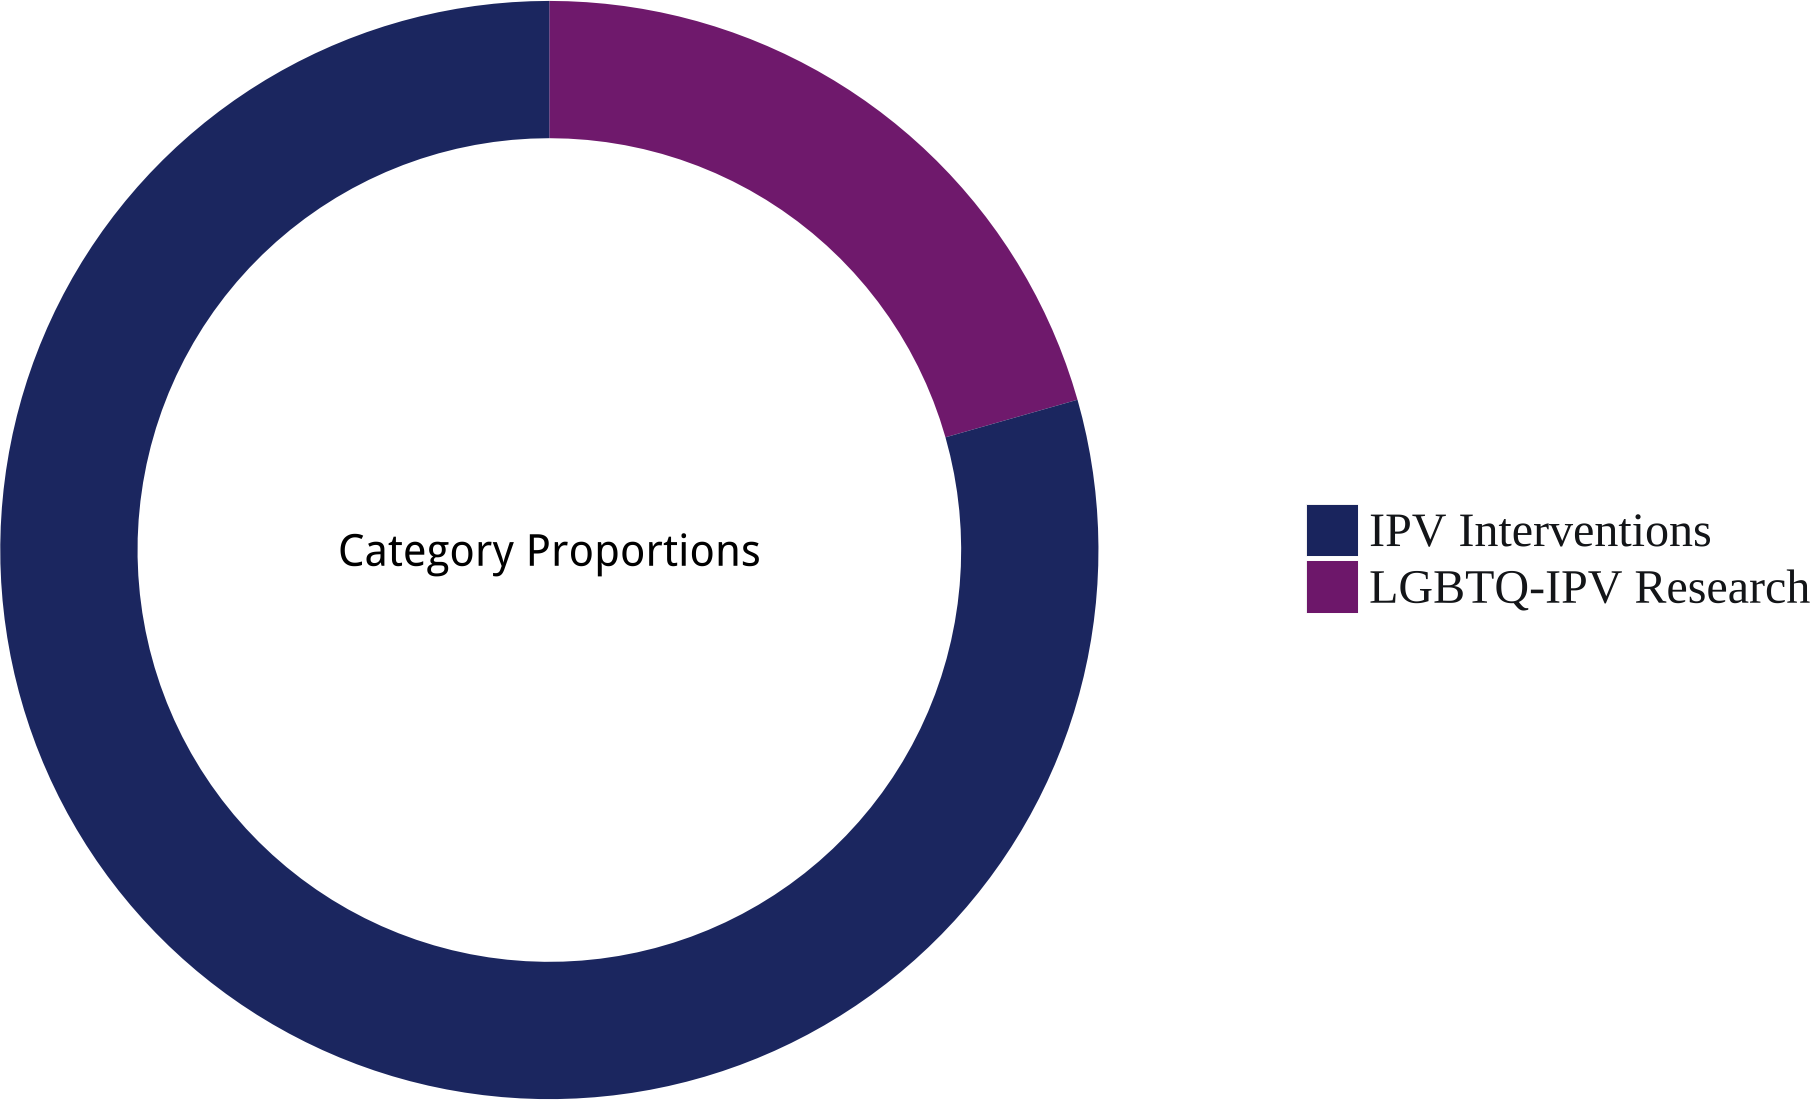
\includegraphics[width=\linewidth]{graphics/rplot-desc-1}

\Reruleb

\section{Publication Titles}\label{publication-titles}

\Rruleb

\begin{Shaded}
\begin{Highlighting}[]
\NormalTok{t.jrnl <-}\StringTok{ }\KeywordTok{Rtdf}\NormalTok{(MAP$journal)}
\NormalTok{ft.jrnl <-}\StringTok{ }\KeywordTok{with}\NormalTok{(MAP, \{}
    \KeywordTok{ftable}\NormalTok{(journal, scat) %>%}\StringTok{ }\KeywordTok{matrix}\NormalTok{(}\DataTypeTok{nrow =} \KeywordTok{nrow}\NormalTok{(t.jrnl), }\DataTypeTok{byrow =} \OtherTok{FALSE}\NormalTok{)}
\NormalTok{\})}
\KeywordTok{dimnames}\NormalTok{(ft.jrnl) <-}\StringTok{ }\KeywordTok{list}\NormalTok{(}\StringTok{`}\DataTypeTok{Publication Title}\StringTok{`} \NormalTok{=}\StringTok{ }\KeywordTok{levels}\NormalTok{(MAP$journal), }
    \DataTypeTok{Category =} \KeywordTok{c}\NormalTok{(}\StringTok{"IPV Interventions"}\NormalTok{, }\StringTok{"LGBTQ-IPV Research"}\NormalTok{))}
\NormalTok{ft.jrnl}
\end{Highlighting}
\end{Shaded}

\begin{longtable}[]{@{}cll@{}}
\toprule
\begin{minipage}[b]{0.49\columnwidth}\centering\strut
~\strut
\end{minipage} & \begin{minipage}[b]{0.21\columnwidth}\raggedright\strut
IPV Interventions\strut
\end{minipage} & \begin{minipage}[b]{0.21\columnwidth}\raggedright\strut
LGBTQ-IPV Research\strut
\end{minipage}\tabularnewline
\midrule
\endhead
\begin{minipage}[t]{0.49\columnwidth}\centering\strut
\textbf{American Journal of Community Psychology}\strut
\end{minipage} & \begin{minipage}[t]{0.21\columnwidth}\raggedright\strut
1\strut
\end{minipage} & \begin{minipage}[t]{0.21\columnwidth}\raggedright\strut
2\strut
\end{minipage}\tabularnewline
\begin{minipage}[t]{0.49\columnwidth}\centering\strut
\textbf{American Journal of Preventive Medicine}\strut
\end{minipage} & \begin{minipage}[t]{0.21\columnwidth}\raggedright\strut
1\strut
\end{minipage} & \begin{minipage}[t]{0.21\columnwidth}\raggedright\strut
0\strut
\end{minipage}\tabularnewline
\begin{minipage}[t]{0.49\columnwidth}\centering\strut
\textbf{American Journal of Public Health}\strut
\end{minipage} & \begin{minipage}[t]{0.21\columnwidth}\raggedright\strut
1\strut
\end{minipage} & \begin{minipage}[t]{0.21\columnwidth}\raggedright\strut
3\strut
\end{minipage}\tabularnewline
\begin{minipage}[t]{0.49\columnwidth}\centering\strut
\textbf{Journal of Interpersonal Violence}\strut
\end{minipage} & \begin{minipage}[t]{0.21\columnwidth}\raggedright\strut
7\strut
\end{minipage} & \begin{minipage}[t]{0.21\columnwidth}\raggedright\strut
17\strut
\end{minipage}\tabularnewline
\begin{minipage}[t]{0.49\columnwidth}\centering\strut
\textbf{Psychology of Women Quarterly}\strut
\end{minipage} & \begin{minipage}[t]{0.21\columnwidth}\raggedright\strut
0\strut
\end{minipage} & \begin{minipage}[t]{0.21\columnwidth}\raggedright\strut
3\strut
\end{minipage}\tabularnewline
\begin{minipage}[t]{0.49\columnwidth}\centering\strut
\textbf{Violence Against Women}\strut
\end{minipage} & \begin{minipage}[t]{0.21\columnwidth}\raggedright\strut
9\strut
\end{minipage} & \begin{minipage}[t]{0.21\columnwidth}\raggedright\strut
10\strut
\end{minipage}\tabularnewline
\begin{minipage}[t]{0.49\columnwidth}\centering\strut
\textbf{Violence and Victims}\strut
\end{minipage} & \begin{minipage}[t]{0.21\columnwidth}\raggedright\strut
4\strut
\end{minipage} & \begin{minipage}[t]{0.21\columnwidth}\raggedright\strut
7\strut
\end{minipage}\tabularnewline
\bottomrule
\end{longtable}

\Reruleb

\newpage

\section{Publication Years}\label{publication-years}

\begin{figure*}
\includegraphics[width=\linewidth]{graphics/rplot-yr_hist1-1} \end{figure*}

\tufteskip

\begin{fullwidth}\begin{centering}



\includegraphics[width=0.85\linewidth]{graphics/rplot-yr_hist2-1} 


\end{centering}\end{fullwidth}

\tufteskip

\newpage

\section{Research Topics, Sampling Frames, and
Methodologies}\label{research-topics-sampling-frames-and-methodologies}

\subsection{Primary Topics}\label{primary-topics}

\begin{longtable}[]{@{}cll@{}}
\toprule
\begin{minipage}[b]{0.47\columnwidth}\centering\strut
~\strut
\end{minipage} & \begin{minipage}[b]{0.22\columnwidth}\raggedright\strut
IPV Interventions\strut
\end{minipage} & \begin{minipage}[b]{0.22\columnwidth}\raggedright\strut
LGBTQ-IPV Research\strut
\end{minipage}\tabularnewline
\midrule
\endhead
\begin{minipage}[t]{0.47\columnwidth}\centering\strut
\textbf{Approach Evaluation}\strut
\end{minipage} & \begin{minipage}[t]{0.22\columnwidth}\raggedright\strut
1\strut
\end{minipage} & \begin{minipage}[t]{0.22\columnwidth}\raggedright\strut
\strut
\end{minipage}\tabularnewline
\begin{minipage}[t]{0.47\columnwidth}\centering\strut
\textbf{Community Capacity}\strut
\end{minipage} & \begin{minipage}[t]{0.22\columnwidth}\raggedright\strut
\strut
\end{minipage} & \begin{minipage}[t]{0.22\columnwidth}\raggedright\strut
1\strut
\end{minipage}\tabularnewline
\begin{minipage}[t]{0.47\columnwidth}\centering\strut
\textbf{Coordinated Community Response}\strut
\end{minipage} & \begin{minipage}[t]{0.22\columnwidth}\raggedright\strut
1\strut
\end{minipage} & \begin{minipage}[t]{0.22\columnwidth}\raggedright\strut
1\strut
\end{minipage}\tabularnewline
\begin{minipage}[t]{0.47\columnwidth}\centering\strut
\textbf{IPV Consequences}\strut
\end{minipage} & \begin{minipage}[t]{0.22\columnwidth}\raggedright\strut
\strut
\end{minipage} & \begin{minipage}[t]{0.22\columnwidth}\raggedright\strut
3\strut
\end{minipage}\tabularnewline
\begin{minipage}[t]{0.47\columnwidth}\centering\strut
\textbf{IPV Dynamics}\strut
\end{minipage} & \begin{minipage}[t]{0.22\columnwidth}\raggedright\strut
\strut
\end{minipage} & \begin{minipage}[t]{0.22\columnwidth}\raggedright\strut
6\strut
\end{minipage}\tabularnewline
\begin{minipage}[t]{0.47\columnwidth}\centering\strut
\textbf{Help-Seeking}\strut
\end{minipage} & \begin{minipage}[t]{0.22\columnwidth}\raggedright\strut
\strut
\end{minipage} & \begin{minipage}[t]{0.22\columnwidth}\raggedright\strut
2\strut
\end{minipage}\tabularnewline
\begin{minipage}[t]{0.47\columnwidth}\centering\strut
\textbf{IPV Interventions (Int.) - General}\strut
\end{minipage} & \begin{minipage}[t]{0.22\columnwidth}\raggedright\strut
\strut
\end{minipage} & \begin{minipage}[t]{0.22\columnwidth}\raggedright\strut
1\strut
\end{minipage}\tabularnewline
\begin{minipage}[t]{0.47\columnwidth}\centering\strut
\textbf{Int. - Description}\strut
\end{minipage} & \begin{minipage}[t]{0.22\columnwidth}\raggedright\strut
2\strut
\end{minipage} & \begin{minipage}[t]{0.22\columnwidth}\raggedright\strut
\strut
\end{minipage}\tabularnewline
\begin{minipage}[t]{0.47\columnwidth}\centering\strut
\textbf{Int. - Proposal}\strut
\end{minipage} & \begin{minipage}[t]{0.22\columnwidth}\raggedright\strut
2\strut
\end{minipage} & \begin{minipage}[t]{0.22\columnwidth}\raggedright\strut
\strut
\end{minipage}\tabularnewline
\begin{minipage}[t]{0.47\columnwidth}\centering\strut
\textbf{Measures}\strut
\end{minipage} & \begin{minipage}[t]{0.22\columnwidth}\raggedright\strut
1\strut
\end{minipage} & \begin{minipage}[t]{0.22\columnwidth}\raggedright\strut
2\strut
\end{minipage}\tabularnewline
\begin{minipage}[t]{0.47\columnwidth}\centering\strut
\textbf{Program Evaluation Methods}\strut
\end{minipage} & \begin{minipage}[t]{0.22\columnwidth}\raggedright\strut
2\strut
\end{minipage} & \begin{minipage}[t]{0.22\columnwidth}\raggedright\strut
\strut
\end{minipage}\tabularnewline
\begin{minipage}[t]{0.47\columnwidth}\centering\strut
\textbf{Perpetrator Characteristics}\strut
\end{minipage} & \begin{minipage}[t]{0.22\columnwidth}\raggedright\strut
\strut
\end{minipage} & \begin{minipage}[t]{0.22\columnwidth}\raggedright\strut
2\strut
\end{minipage}\tabularnewline
\begin{minipage}[t]{0.47\columnwidth}\centering\strut
\textbf{Program/Policy Development}\strut
\end{minipage} & \begin{minipage}[t]{0.22\columnwidth}\raggedright\strut
3\strut
\end{minipage} & \begin{minipage}[t]{0.22\columnwidth}\raggedright\strut
\strut
\end{minipage}\tabularnewline
\begin{minipage}[t]{0.47\columnwidth}\centering\strut
\textbf{Outsiders' Perspectives}\strut
\end{minipage} & \begin{minipage}[t]{0.22\columnwidth}\raggedright\strut
\strut
\end{minipage} & \begin{minipage}[t]{0.22\columnwidth}\raggedright\strut
6\strut
\end{minipage}\tabularnewline
\begin{minipage}[t]{0.47\columnwidth}\centering\strut
\textbf{Intervention Providers' Perspectives}\strut
\end{minipage} & \begin{minipage}[t]{0.22\columnwidth}\raggedright\strut
1\strut
\end{minipage} & \begin{minipage}[t]{0.22\columnwidth}\raggedright\strut
\strut
\end{minipage}\tabularnewline
\begin{minipage}[t]{0.47\columnwidth}\centering\strut
\textbf{Key Stakeholders' Persepctives}\strut
\end{minipage} & \begin{minipage}[t]{0.22\columnwidth}\raggedright\strut
\strut
\end{minipage} & \begin{minipage}[t]{0.22\columnwidth}\raggedright\strut
1\strut
\end{minipage}\tabularnewline
\begin{minipage}[t]{0.47\columnwidth}\centering\strut
\textbf{Victims'/Survivors' Perspectives}\strut
\end{minipage} & \begin{minipage}[t]{0.22\columnwidth}\raggedright\strut
2\strut
\end{minipage} & \begin{minipage}[t]{0.22\columnwidth}\raggedright\strut
1\strut
\end{minipage}\tabularnewline
\begin{minipage}[t]{0.47\columnwidth}\centering\strut
\textbf{Program/Policy Evaluation - General}\strut
\end{minipage} & \begin{minipage}[t]{0.22\columnwidth}\raggedright\strut
18\strut
\end{minipage} & \begin{minipage}[t]{0.22\columnwidth}\raggedright\strut
\strut
\end{minipage}\tabularnewline
\begin{minipage}[t]{0.47\columnwidth}\centering\strut
\textbf{Protective Factors}\strut
\end{minipage} & \begin{minipage}[t]{0.22\columnwidth}\raggedright\strut
\strut
\end{minipage} & \begin{minipage}[t]{0.22\columnwidth}\raggedright\strut
1\strut
\end{minipage}\tabularnewline
\begin{minipage}[t]{0.47\columnwidth}\centering\strut
\textbf{Public Policy}\strut
\end{minipage} & \begin{minipage}[t]{0.22\columnwidth}\raggedright\strut
2\strut
\end{minipage} & \begin{minipage}[t]{0.22\columnwidth}\raggedright\strut
\strut
\end{minipage}\tabularnewline
\begin{minipage}[t]{0.47\columnwidth}\centering\strut
\textbf{IPV Prevalence}\strut
\end{minipage} & \begin{minipage}[t]{0.22\columnwidth}\raggedright\strut
\strut
\end{minipage} & \begin{minipage}[t]{0.22\columnwidth}\raggedright\strut
13\strut
\end{minipage}\tabularnewline
\begin{minipage}[t]{0.47\columnwidth}\centering\strut
\textbf{Risk Factors}\strut
\end{minipage} & \begin{minipage}[t]{0.22\columnwidth}\raggedright\strut
\strut
\end{minipage} & \begin{minipage}[t]{0.22\columnwidth}\raggedright\strut
15\strut
\end{minipage}\tabularnewline
\begin{minipage}[t]{0.47\columnwidth}\centering\strut
\textbf{System Response}\strut
\end{minipage} & \begin{minipage}[t]{0.22\columnwidth}\raggedright\strut
2\strut
\end{minipage} & \begin{minipage}[t]{0.22\columnwidth}\raggedright\strut
2\strut
\end{minipage}\tabularnewline
\bottomrule
\end{longtable}

\begin{longtable}[]{@{}cl@{}}
\toprule
\begin{minipage}[b]{0.56\columnwidth}\centering\strut
~\strut
\end{minipage} & \begin{minipage}[b]{0.16\columnwidth}\raggedright\strut
dfm.tp2.s3\strut
\end{minipage}\tabularnewline
\midrule
\endhead
\begin{minipage}[t]{0.56\columnwidth}\centering\strut
\textbf{Approach Evaluation}\strut
\end{minipage} & \begin{minipage}[t]{0.16\columnwidth}\raggedright\strut
1\strut
\end{minipage}\tabularnewline
\begin{minipage}[t]{0.56\columnwidth}\centering\strut
\textbf{Coordinated Community Response}\strut
\end{minipage} & \begin{minipage}[t]{0.16\columnwidth}\raggedright\strut
1\strut
\end{minipage}\tabularnewline
\begin{minipage}[t]{0.56\columnwidth}\centering\strut
\textbf{Int. - Description}\strut
\end{minipage} & \begin{minipage}[t]{0.16\columnwidth}\raggedright\strut
2\strut
\end{minipage}\tabularnewline
\begin{minipage}[t]{0.56\columnwidth}\centering\strut
\textbf{Int. - Proposal}\strut
\end{minipage} & \begin{minipage}[t]{0.16\columnwidth}\raggedright\strut
2\strut
\end{minipage}\tabularnewline
\begin{minipage}[t]{0.56\columnwidth}\centering\strut
\textbf{Measures}\strut
\end{minipage} & \begin{minipage}[t]{0.16\columnwidth}\raggedright\strut
1\strut
\end{minipage}\tabularnewline
\begin{minipage}[t]{0.56\columnwidth}\centering\strut
\textbf{Program Evaluation Methods}\strut
\end{minipage} & \begin{minipage}[t]{0.16\columnwidth}\raggedright\strut
2\strut
\end{minipage}\tabularnewline
\begin{minipage}[t]{0.56\columnwidth}\centering\strut
\textbf{Program/Policy Development}\strut
\end{minipage} & \begin{minipage}[t]{0.16\columnwidth}\raggedright\strut
3\strut
\end{minipage}\tabularnewline
\begin{minipage}[t]{0.56\columnwidth}\centering\strut
\textbf{Intervention Providers' Perspectives}\strut
\end{minipage} & \begin{minipage}[t]{0.16\columnwidth}\raggedright\strut
1\strut
\end{minipage}\tabularnewline
\begin{minipage}[t]{0.56\columnwidth}\centering\strut
\textbf{Victims'/Survivors' Perspectives}\strut
\end{minipage} & \begin{minipage}[t]{0.16\columnwidth}\raggedright\strut
2\strut
\end{minipage}\tabularnewline
\begin{minipage}[t]{0.56\columnwidth}\centering\strut
\textbf{Program/Policy Evaluation - General}\strut
\end{minipage} & \begin{minipage}[t]{0.16\columnwidth}\raggedright\strut
18\strut
\end{minipage}\tabularnewline
\begin{minipage}[t]{0.56\columnwidth}\centering\strut
\textbf{Public Policy}\strut
\end{minipage} & \begin{minipage}[t]{0.16\columnwidth}\raggedright\strut
2\strut
\end{minipage}\tabularnewline
\begin{minipage}[t]{0.56\columnwidth}\centering\strut
\textbf{System Response}\strut
\end{minipage} & \begin{minipage}[t]{0.16\columnwidth}\raggedright\strut
2\strut
\end{minipage}\tabularnewline
\bottomrule
\end{longtable}

\begin{longtable}[]{@{}cl@{}}
\toprule
\begin{minipage}[b]{0.54\columnwidth}\centering\strut
~\strut
\end{minipage} & \begin{minipage}[b]{0.16\columnwidth}\raggedright\strut
dfm.tp2.s4\strut
\end{minipage}\tabularnewline
\midrule
\endhead
\begin{minipage}[t]{0.54\columnwidth}\centering\strut
\textbf{Community Capacity}\strut
\end{minipage} & \begin{minipage}[t]{0.16\columnwidth}\raggedright\strut
1\strut
\end{minipage}\tabularnewline
\begin{minipage}[t]{0.54\columnwidth}\centering\strut
\textbf{Coordinated Community Response}\strut
\end{minipage} & \begin{minipage}[t]{0.16\columnwidth}\raggedright\strut
1\strut
\end{minipage}\tabularnewline
\begin{minipage}[t]{0.54\columnwidth}\centering\strut
\textbf{IPV Consequences}\strut
\end{minipage} & \begin{minipage}[t]{0.16\columnwidth}\raggedright\strut
3\strut
\end{minipage}\tabularnewline
\begin{minipage}[t]{0.54\columnwidth}\centering\strut
\textbf{IPV Dynamics}\strut
\end{minipage} & \begin{minipage}[t]{0.16\columnwidth}\raggedright\strut
6\strut
\end{minipage}\tabularnewline
\begin{minipage}[t]{0.54\columnwidth}\centering\strut
\textbf{Help-Seeking}\strut
\end{minipage} & \begin{minipage}[t]{0.16\columnwidth}\raggedright\strut
2\strut
\end{minipage}\tabularnewline
\begin{minipage}[t]{0.54\columnwidth}\centering\strut
\textbf{IPV Interventions (Int.) - General}\strut
\end{minipage} & \begin{minipage}[t]{0.16\columnwidth}\raggedright\strut
1\strut
\end{minipage}\tabularnewline
\begin{minipage}[t]{0.54\columnwidth}\centering\strut
\textbf{Measures}\strut
\end{minipage} & \begin{minipage}[t]{0.16\columnwidth}\raggedright\strut
2\strut
\end{minipage}\tabularnewline
\begin{minipage}[t]{0.54\columnwidth}\centering\strut
\textbf{Perpetrator Characteristics}\strut
\end{minipage} & \begin{minipage}[t]{0.16\columnwidth}\raggedright\strut
2\strut
\end{minipage}\tabularnewline
\begin{minipage}[t]{0.54\columnwidth}\centering\strut
\textbf{Outsiders' Perspectives}\strut
\end{minipage} & \begin{minipage}[t]{0.16\columnwidth}\raggedright\strut
6\strut
\end{minipage}\tabularnewline
\begin{minipage}[t]{0.54\columnwidth}\centering\strut
\textbf{Key Stakeholders' Persepctives}\strut
\end{minipage} & \begin{minipage}[t]{0.16\columnwidth}\raggedright\strut
1\strut
\end{minipage}\tabularnewline
\begin{minipage}[t]{0.54\columnwidth}\centering\strut
\textbf{Victims'/Survivors' Perspectives}\strut
\end{minipage} & \begin{minipage}[t]{0.16\columnwidth}\raggedright\strut
1\strut
\end{minipage}\tabularnewline
\begin{minipage}[t]{0.54\columnwidth}\centering\strut
\textbf{Protective Factors}\strut
\end{minipage} & \begin{minipage}[t]{0.16\columnwidth}\raggedright\strut
1\strut
\end{minipage}\tabularnewline
\begin{minipage}[t]{0.54\columnwidth}\centering\strut
\textbf{IPV Prevalence}\strut
\end{minipage} & \begin{minipage}[t]{0.16\columnwidth}\raggedright\strut
13\strut
\end{minipage}\tabularnewline
\begin{minipage}[t]{0.54\columnwidth}\centering\strut
\textbf{Risk Factors}\strut
\end{minipage} & \begin{minipage}[t]{0.16\columnwidth}\raggedright\strut
15\strut
\end{minipage}\tabularnewline
\begin{minipage}[t]{0.54\columnwidth}\centering\strut
\textbf{System Response}\strut
\end{minipage} & \begin{minipage}[t]{0.16\columnwidth}\raggedright\strut
2\strut
\end{minipage}\tabularnewline
\bottomrule
\end{longtable}

\begin{figure*}
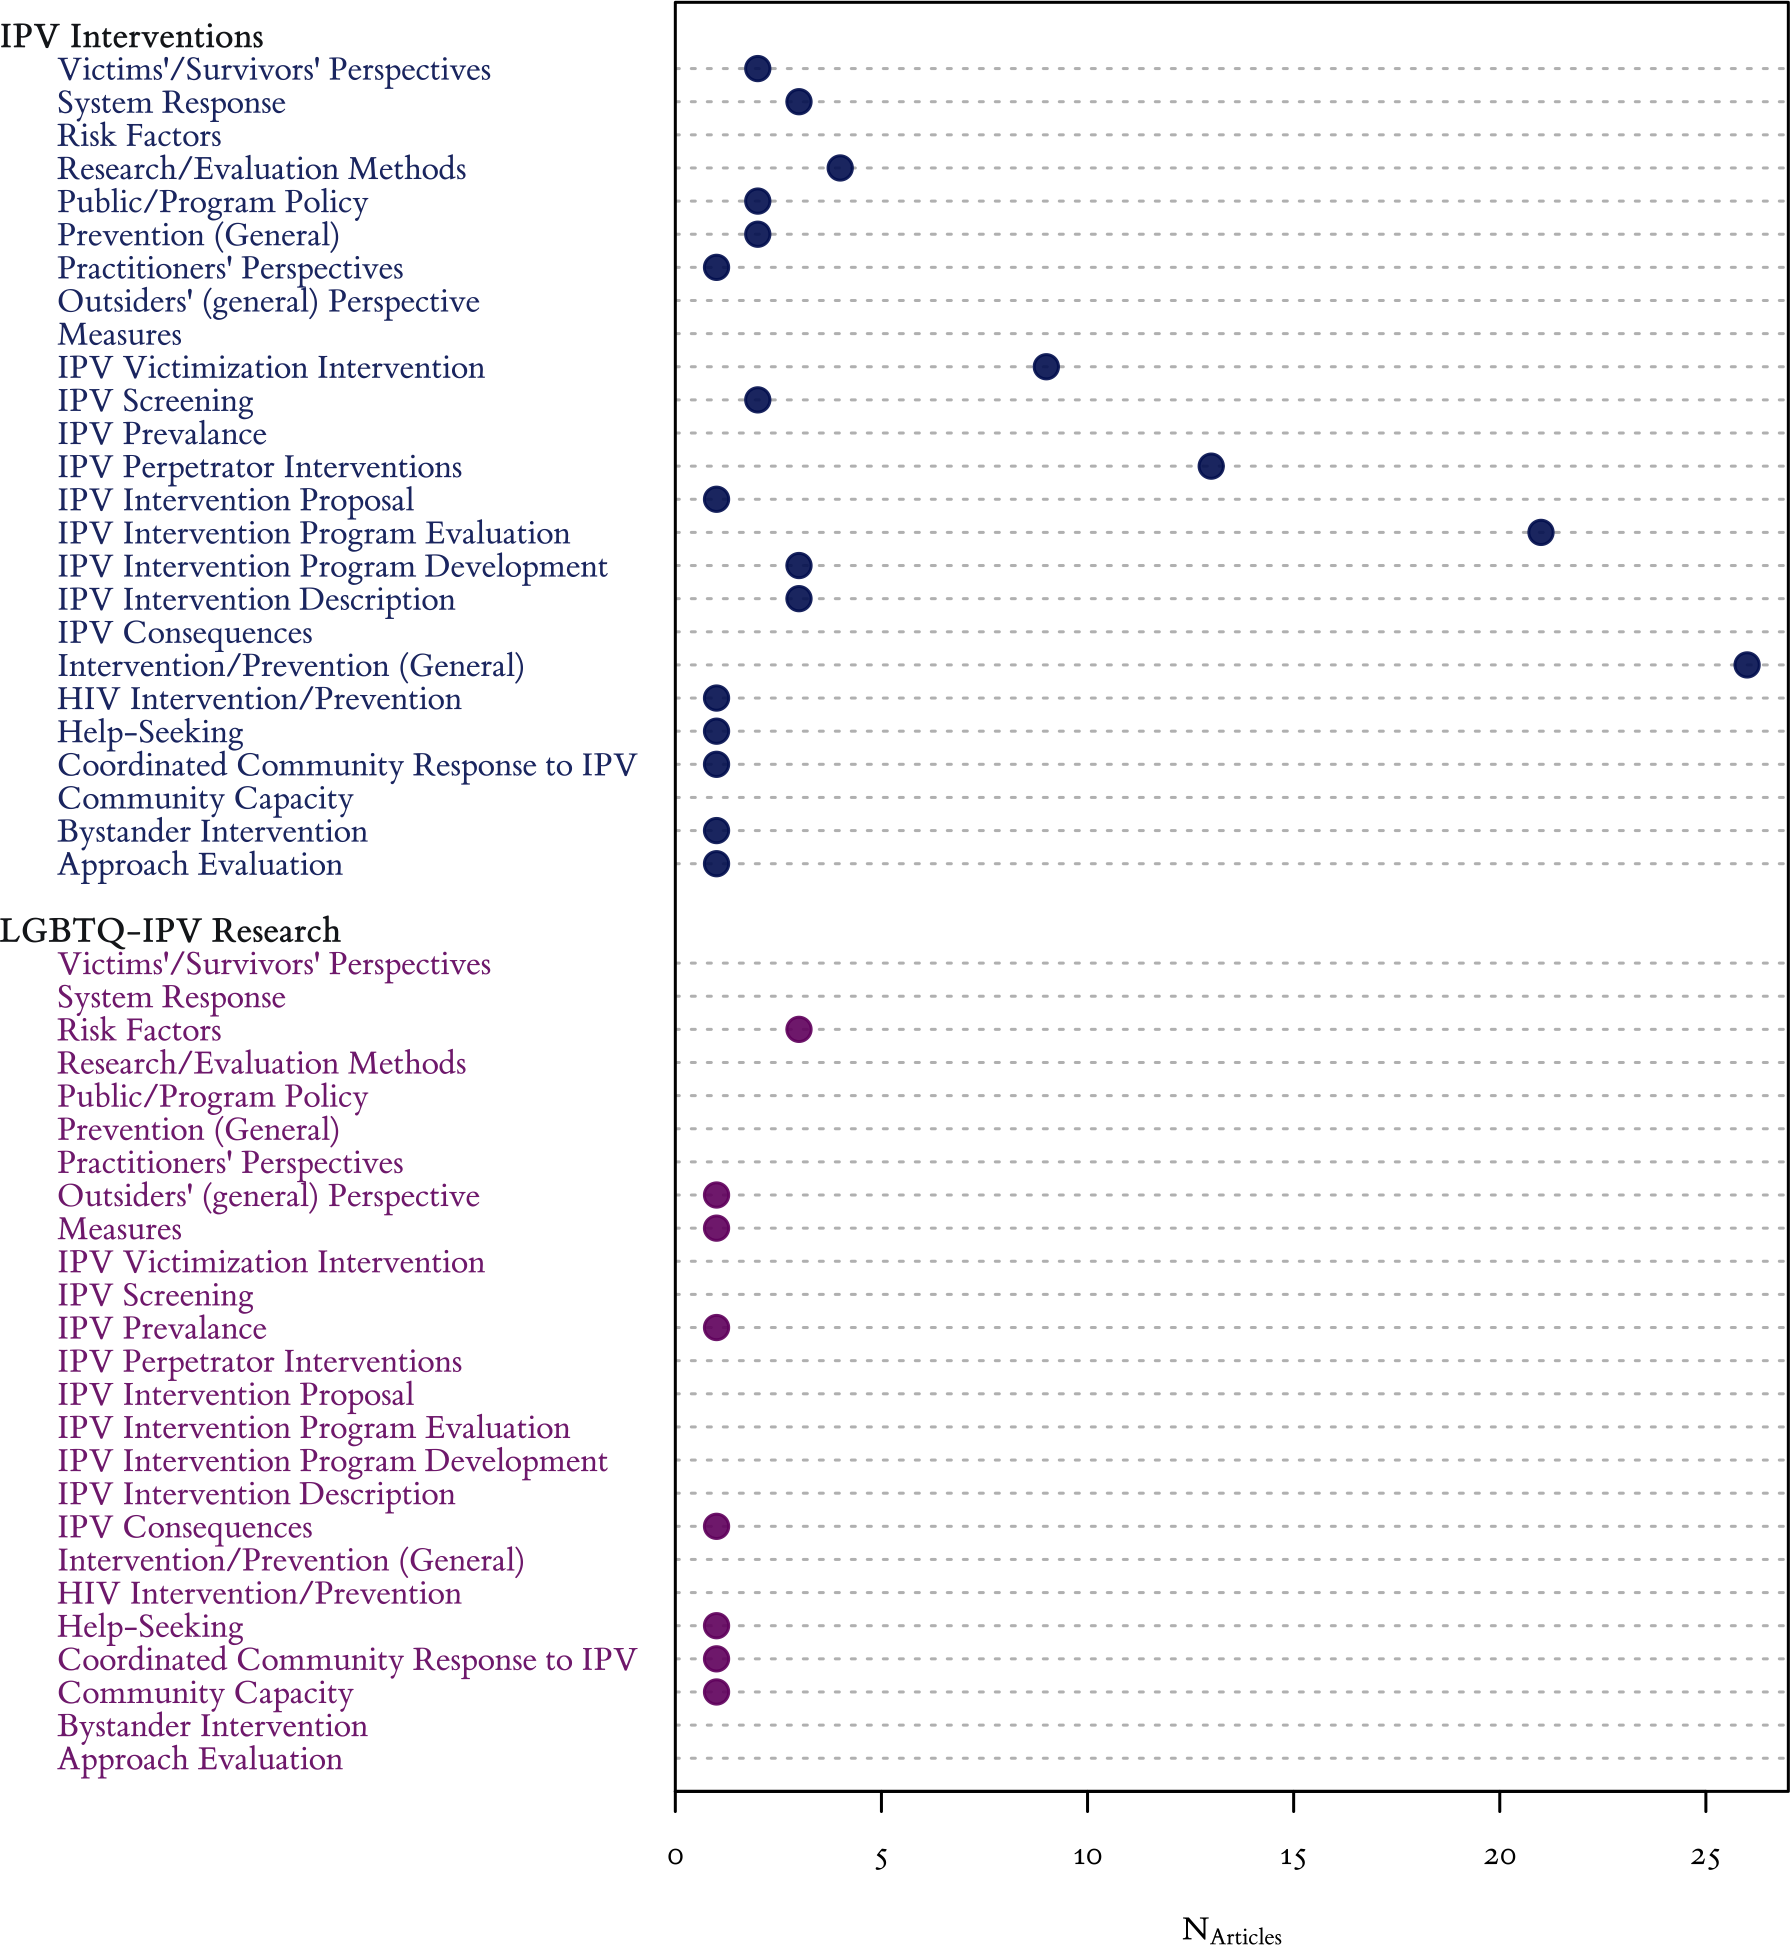
\includegraphics[width=\linewidth]{graphics/rplot-topics-1} \includegraphics[width=\linewidth]{graphics/rplot-topics-2} \end{figure*}

\subsection{Methodologies}\label{methodologies}

\begin{longtable}[]{@{}ll@{}}
\toprule
\begin{minipage}[b]{0.21\columnwidth}\raggedright\strut
Method(s)\strut
\end{minipage} & \begin{minipage}[b]{0.21\columnwidth}\raggedright\strut
\(N_{Articles}\)\strut
\end{minipage}\tabularnewline
\midrule
\endhead
\begin{minipage}[t]{0.21\columnwidth}\raggedright\strut
Mixed-Methods\strut
\end{minipage} & \begin{minipage}[t]{0.21\columnwidth}\raggedright\strut
8\strut
\end{minipage}\tabularnewline
\begin{minipage}[t]{0.21\columnwidth}\raggedright\strut
Qualitative\strut
\end{minipage} & \begin{minipage}[t]{0.21\columnwidth}\raggedright\strut
14\strut
\end{minipage}\tabularnewline
\begin{minipage}[t]{0.21\columnwidth}\raggedright\strut
Quantitative\strut
\end{minipage} & \begin{minipage}[t]{0.21\columnwidth}\raggedright\strut
42\strut
\end{minipage}\tabularnewline
\bottomrule
\end{longtable}

\begin{longtable}[]{@{}cll@{}}
\toprule
\begin{minipage}[b]{0.25\columnwidth}\centering\strut
~\strut
\end{minipage} & \begin{minipage}[b]{0.25\columnwidth}\raggedright\strut
IPV Interventions\strut
\end{minipage} & \begin{minipage}[b]{0.25\columnwidth}\raggedright\strut
LGBTQ-IPV Research\strut
\end{minipage}\tabularnewline
\midrule
\endhead
\begin{minipage}[t]{0.25\columnwidth}\centering\strut
\textbf{Mixed-Methods}\strut
\end{minipage} & \begin{minipage}[t]{0.25\columnwidth}\raggedright\strut
2\strut
\end{minipage} & \begin{minipage}[t]{0.25\columnwidth}\raggedright\strut
6\strut
\end{minipage}\tabularnewline
\begin{minipage}[t]{0.25\columnwidth}\centering\strut
\textbf{Qualitative}\strut
\end{minipage} & \begin{minipage}[t]{0.25\columnwidth}\raggedright\strut
6\strut
\end{minipage} & \begin{minipage}[t]{0.25\columnwidth}\raggedright\strut
8\strut
\end{minipage}\tabularnewline
\begin{minipage}[t]{0.25\columnwidth}\centering\strut
\textbf{Quantitative}\strut
\end{minipage} & \begin{minipage}[t]{0.25\columnwidth}\raggedright\strut
14\strut
\end{minipage} & \begin{minipage}[t]{0.25\columnwidth}\raggedright\strut
28\strut
\end{minipage}\tabularnewline
\bottomrule
\end{longtable}

\begin{figure*}
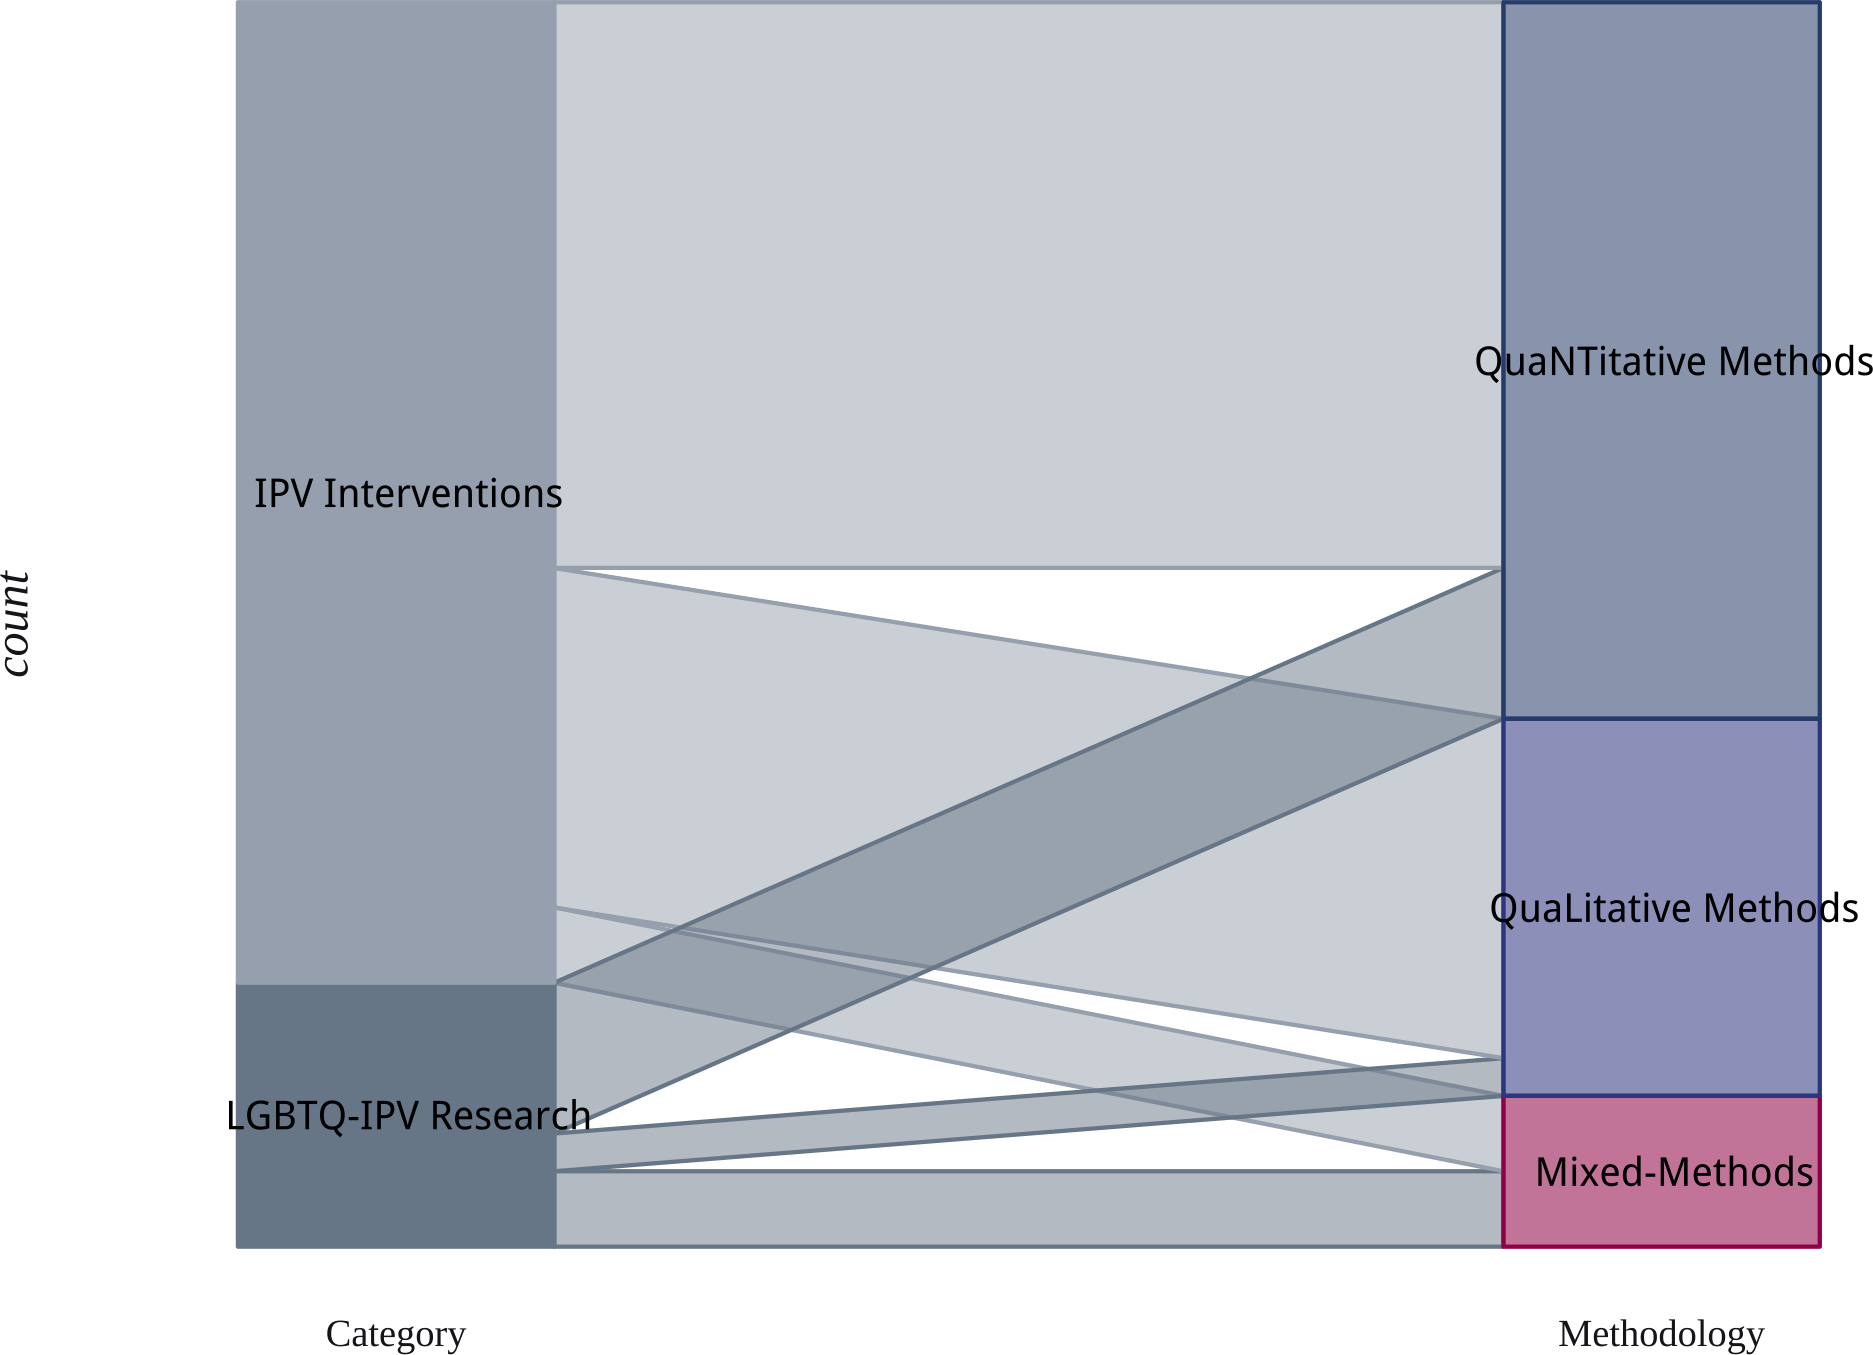
\includegraphics[width=\linewidth]{graphics/rplot-methodologies-1} \includegraphics[width=\linewidth]{graphics/rplot-methodologies-2} \end{figure*}

\newpage

\newthought{\large{Qualitative Methods}}

\begin{longtable}[]{@{}ll@{}}
\toprule
\begin{minipage}[b]{0.41\columnwidth}\raggedright\strut
Qualitative Method(s)\strut
\end{minipage} & \begin{minipage}[b]{0.21\columnwidth}\raggedright\strut
\(N_{Articles}\)\strut
\end{minipage}\tabularnewline
\midrule
\endhead
\begin{minipage}[t]{0.41\columnwidth}\raggedright\strut
Case Study\strut
\end{minipage} & \begin{minipage}[t]{0.21\columnwidth}\raggedright\strut
1\strut
\end{minipage}\tabularnewline
\begin{minipage}[t]{0.41\columnwidth}\raggedright\strut
Focus Groups\strut
\end{minipage} & \begin{minipage}[t]{0.21\columnwidth}\raggedright\strut
2\strut
\end{minipage}\tabularnewline
\begin{minipage}[t]{0.41\columnwidth}\raggedright\strut
Group Interviews\strut
\end{minipage} & \begin{minipage}[t]{0.21\columnwidth}\raggedright\strut
10\strut
\end{minipage}\tabularnewline
\begin{minipage}[t]{0.41\columnwidth}\raggedright\strut
1-on-1 Interviews\strut
\end{minipage} & \begin{minipage}[t]{0.21\columnwidth}\raggedright\strut
1\strut
\end{minipage}\tabularnewline
\begin{minipage}[t]{0.41\columnwidth}\raggedright\strut
Multiple Qualitative Methods\strut
\end{minipage} & \begin{minipage}[t]{0.21\columnwidth}\raggedright\strut
2\strut
\end{minipage}\tabularnewline
\begin{minipage}[t]{0.41\columnwidth}\raggedright\strut
Qualitative Survey\strut
\end{minipage} & \begin{minipage}[t]{0.21\columnwidth}\raggedright\strut
1\strut
\end{minipage}\tabularnewline
\bottomrule
\end{longtable}

\begin{figure*}
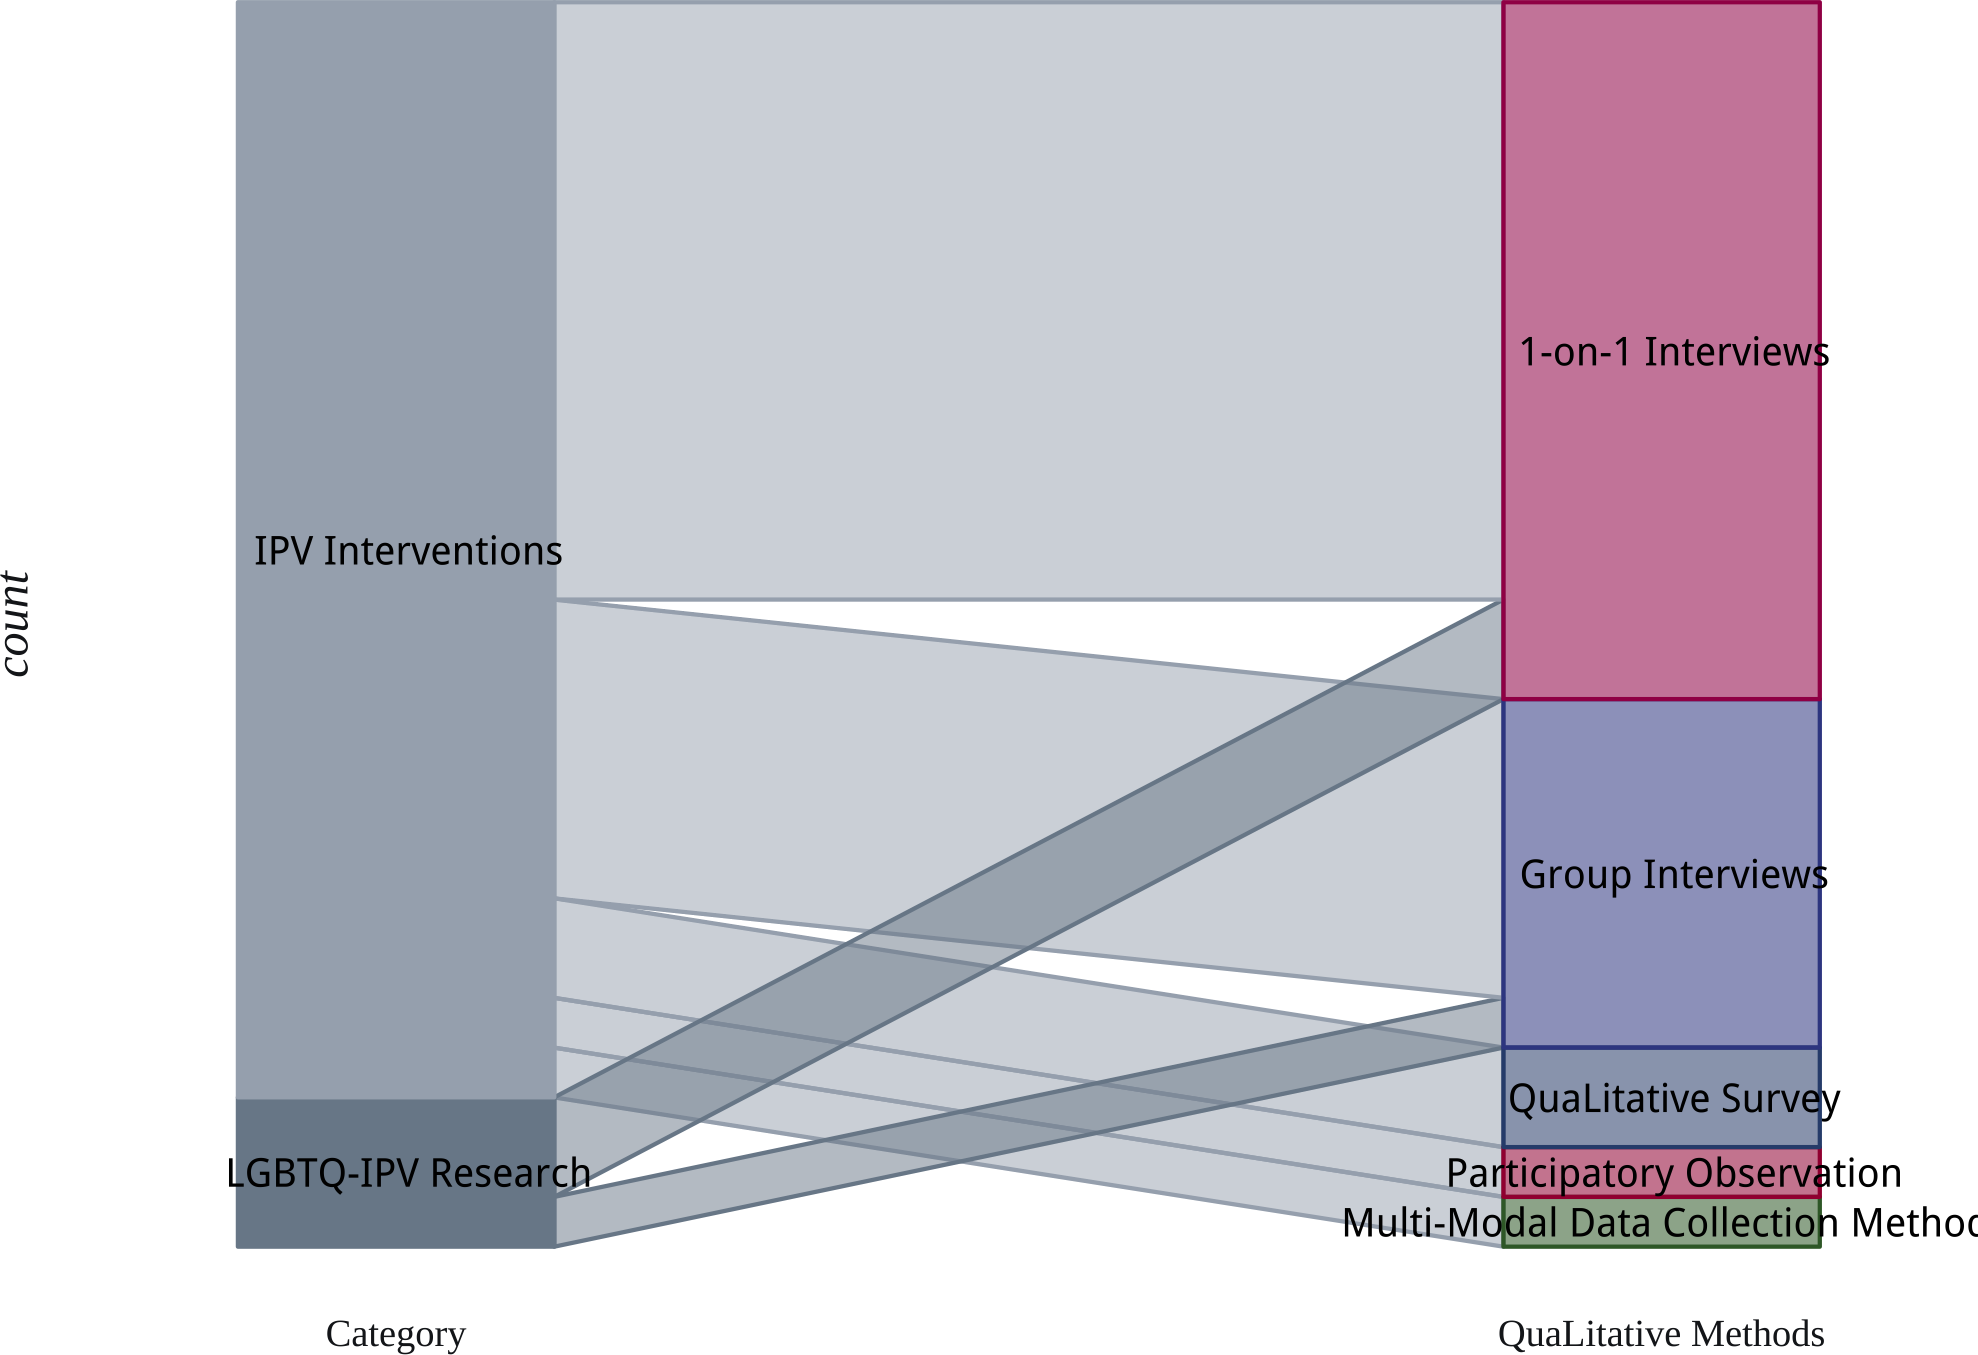
\includegraphics[width=\linewidth]{graphics/rplot-qual-1} \includegraphics[width=\linewidth]{graphics/rplot-qual-2} \end{figure*}

\newpage

\newthought{\large{Quantitative Methods}}

\begin{longtable}[]{@{}ll@{}}
\toprule
\begin{minipage}[b]{0.51\columnwidth}\raggedright\strut
Quantitative Method\strut
\end{minipage} & \begin{minipage}[b]{0.21\columnwidth}\raggedright\strut
\(N_{Articles}\)\strut
\end{minipage}\tabularnewline
\midrule
\endhead
\begin{minipage}[t]{0.51\columnwidth}\raggedright\strut
Secondary/Archival Data\strut
\end{minipage} & \begin{minipage}[t]{0.21\columnwidth}\raggedright\strut
10\strut
\end{minipage}\tabularnewline
\begin{minipage}[t]{0.51\columnwidth}\raggedright\strut
Experimental Design\strut
\end{minipage} & \begin{minipage}[t]{0.21\columnwidth}\raggedright\strut
13\strut
\end{minipage}\tabularnewline
\begin{minipage}[t]{0.51\columnwidth}\raggedright\strut
Longitudinal\strut
\end{minipage} & \begin{minipage}[t]{0.21\columnwidth}\raggedright\strut
12\strut
\end{minipage}\tabularnewline
\begin{minipage}[t]{0.51\columnwidth}\raggedright\strut
Multiple Quantitative Methods\strut
\end{minipage} & \begin{minipage}[t]{0.21\columnwidth}\raggedright\strut
2\strut
\end{minipage}\tabularnewline
\begin{minipage}[t]{0.51\columnwidth}\raggedright\strut
Intervention Providers' Perspectives\strut
\end{minipage} & \begin{minipage}[t]{0.21\columnwidth}\raggedright\strut
1\strut
\end{minipage}\tabularnewline
\begin{minipage}[t]{0.51\columnwidth}\raggedright\strut
Client Records\strut
\end{minipage} & \begin{minipage}[t]{0.21\columnwidth}\raggedright\strut
3\strut
\end{minipage}\tabularnewline
\begin{minipage}[t]{0.51\columnwidth}\raggedright\strut
Police Records\strut
\end{minipage} & \begin{minipage}[t]{0.21\columnwidth}\raggedright\strut
5\strut
\end{minipage}\tabularnewline
\begin{minipage}[t]{0.51\columnwidth}\raggedright\strut
Quantitative Survey\strut
\end{minipage} & \begin{minipage}[t]{0.21\columnwidth}\raggedright\strut
39\strut
\end{minipage}\tabularnewline
\begin{minipage}[t]{0.51\columnwidth}\raggedright\strut
Cross-Sectional\strut
\end{minipage} & \begin{minipage}[t]{0.21\columnwidth}\raggedright\strut
29\strut
\end{minipage}\tabularnewline
\bottomrule
\end{longtable}

\begin{figure*}
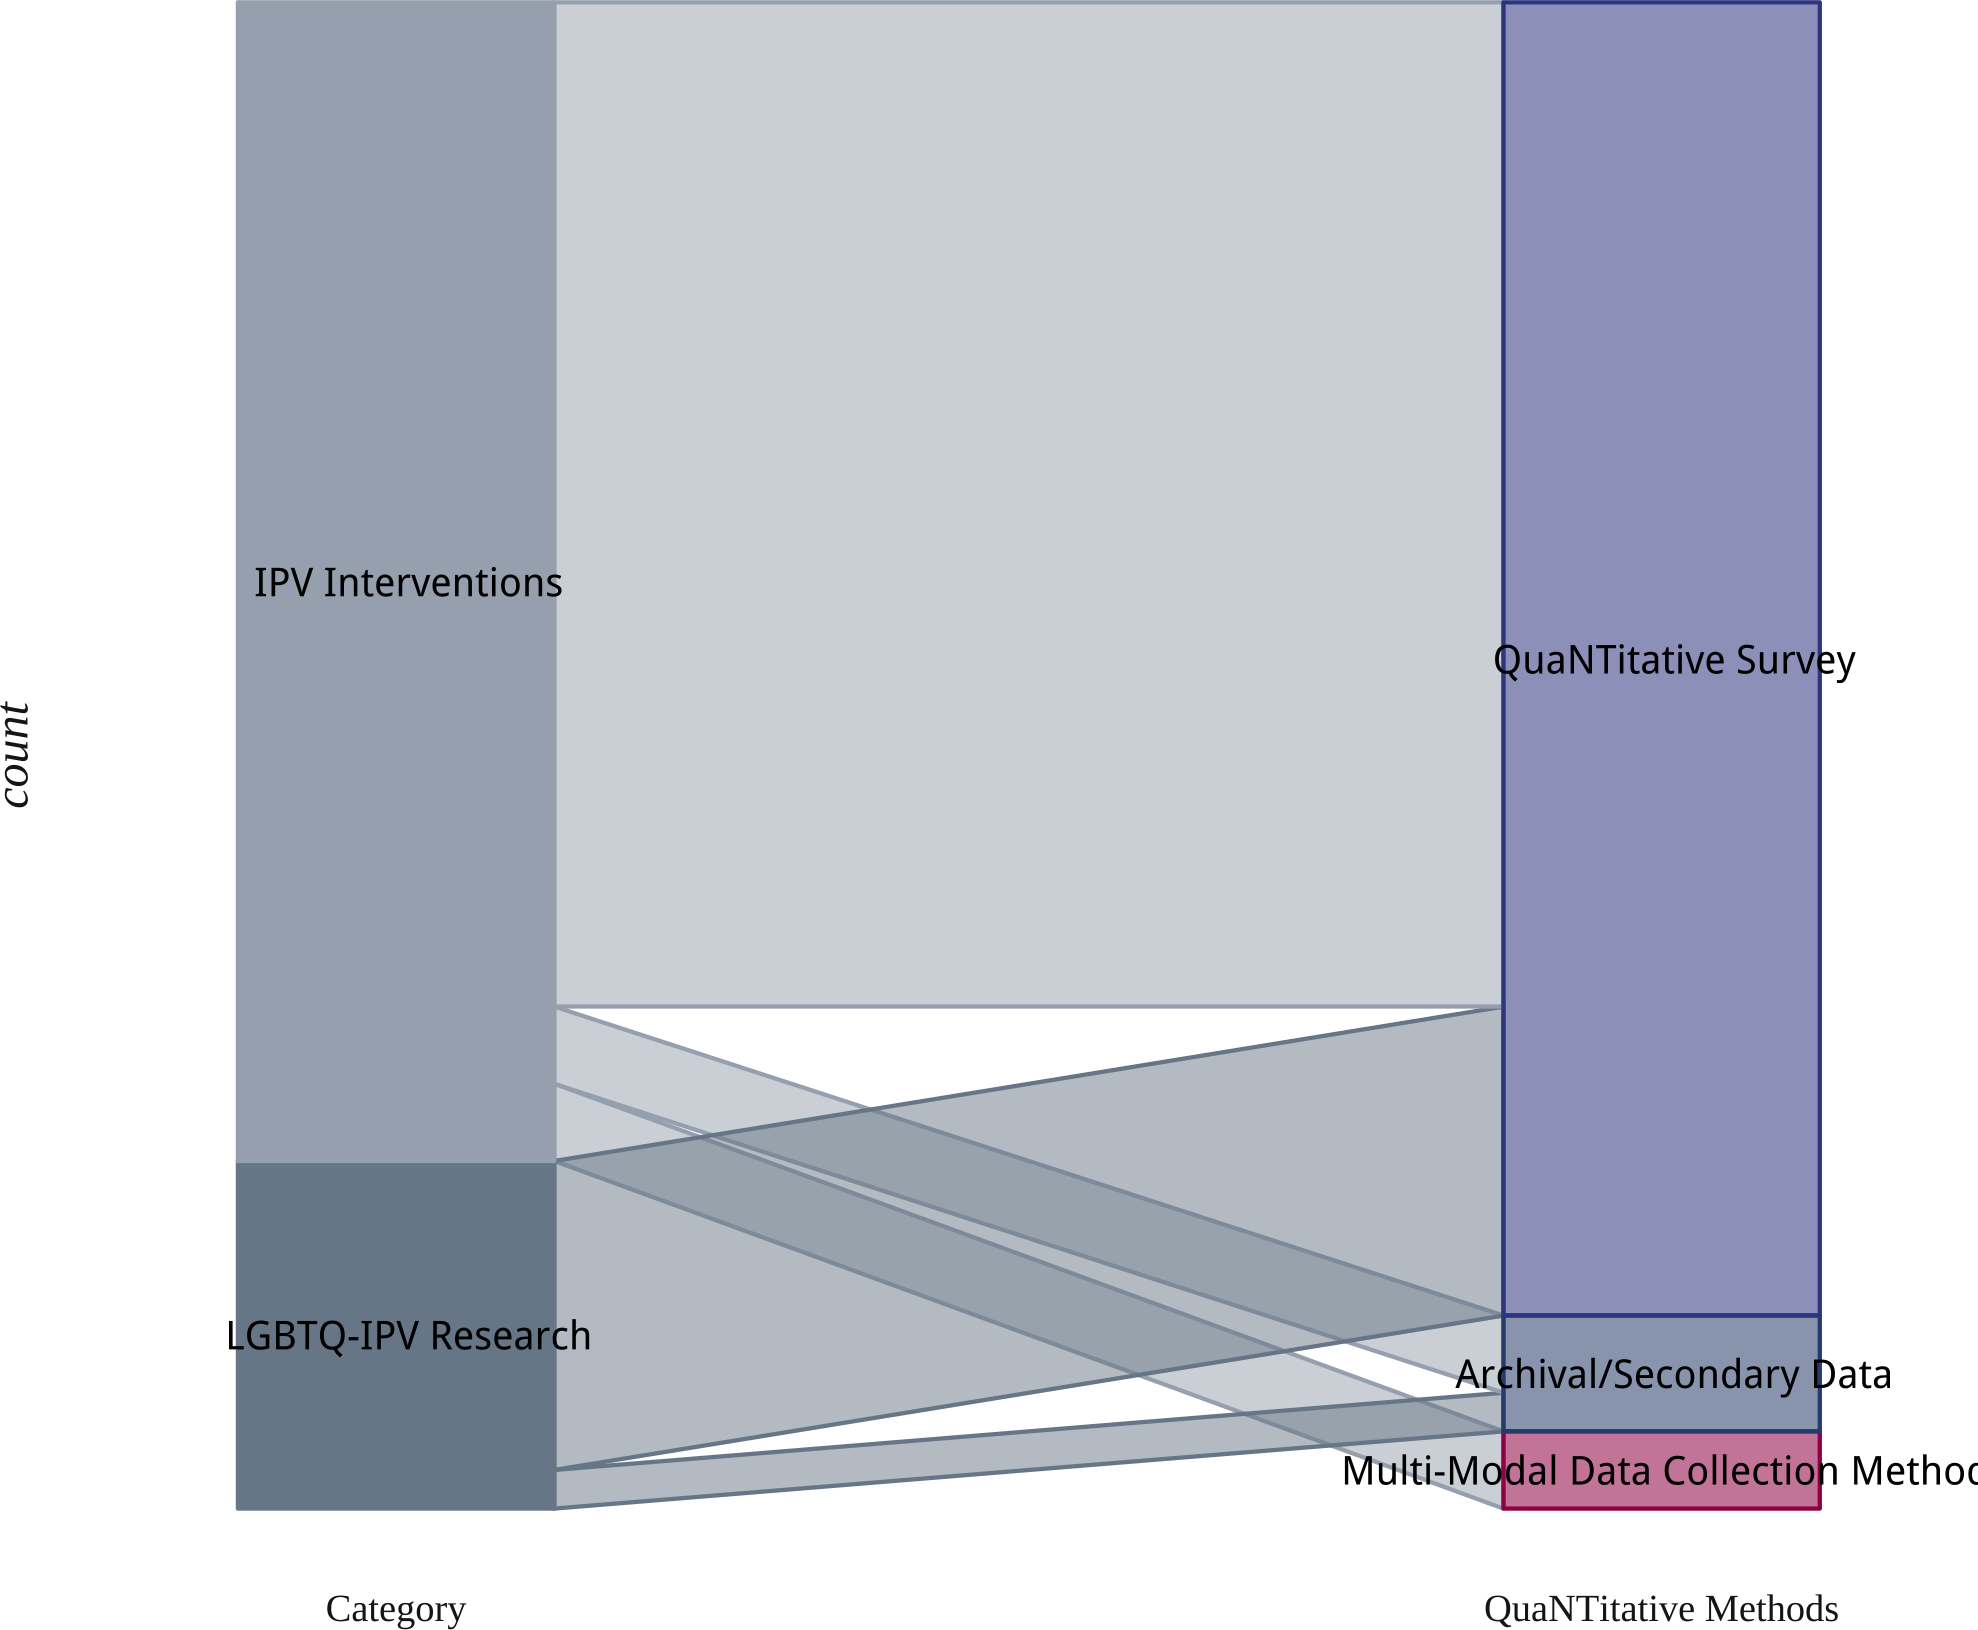
\includegraphics[width=\linewidth]{graphics/rplot-quant-1} \includegraphics[width=\linewidth]{graphics/rplot-quant-2} \end{figure*}

\newpage

\newthought{\large{Mixed-Methods}}

\begin{longtable}[]{@{}ll@{}}
\toprule
\begin{minipage}[b]{0.29\columnwidth}\raggedright\strut
Methods\strut
\end{minipage} & \begin{minipage}[b]{0.21\columnwidth}\raggedright\strut
\(N_{Articles}\)\strut
\end{minipage}\tabularnewline
\midrule
\endhead
\begin{minipage}[t]{0.29\columnwidth}\raggedright\strut
Experimental Design\strut
\end{minipage} & \begin{minipage}[t]{0.21\columnwidth}\raggedright\strut
2\strut
\end{minipage}\tabularnewline
\begin{minipage}[t]{0.29\columnwidth}\raggedright\strut
Focus Groups\strut
\end{minipage} & \begin{minipage}[t]{0.21\columnwidth}\raggedright\strut
6\strut
\end{minipage}\tabularnewline
\begin{minipage}[t]{0.29\columnwidth}\raggedright\strut
Group Interviews\strut
\end{minipage} & \begin{minipage}[t]{0.21\columnwidth}\raggedright\strut
2\strut
\end{minipage}\tabularnewline
\begin{minipage}[t]{0.29\columnwidth}\raggedright\strut
Longitudinal\strut
\end{minipage} & \begin{minipage}[t]{0.21\columnwidth}\raggedright\strut
3\strut
\end{minipage}\tabularnewline
\begin{minipage}[t]{0.29\columnwidth}\raggedright\strut
Qualitative Survey\strut
\end{minipage} & \begin{minipage}[t]{0.21\columnwidth}\raggedright\strut
2\strut
\end{minipage}\tabularnewline
\begin{minipage}[t]{0.29\columnwidth}\raggedright\strut
Quantitative Survey\strut
\end{minipage} & \begin{minipage}[t]{0.21\columnwidth}\raggedright\strut
8\strut
\end{minipage}\tabularnewline
\begin{minipage}[t]{0.29\columnwidth}\raggedright\strut
Cross-Sectional\strut
\end{minipage} & \begin{minipage}[t]{0.21\columnwidth}\raggedright\strut
2\strut
\end{minipage}\tabularnewline
\bottomrule
\end{longtable}

\begin{figure*}
\includegraphics[width=\linewidth]{graphics/rplot-mixed-1} \includegraphics[width=\linewidth]{graphics/rplot-mixed-2} \end{figure*}

\newpage

\newthought{\large{Populations}}

\begin{longtable}[]{@{}ll@{}}
\toprule
\begin{minipage}[b]{0.59\columnwidth}\raggedright\strut
Population\strut
\end{minipage} & \begin{minipage}[b]{0.21\columnwidth}\raggedright\strut
\(N_{Articles}\)\strut
\end{minipage}\tabularnewline
\midrule
\endhead
\begin{minipage}[t]{0.59\columnwidth}\raggedright\strut
African Americans\strut
\end{minipage} & \begin{minipage}[t]{0.21\columnwidth}\raggedright\strut
2\strut
\end{minipage}\tabularnewline
\begin{minipage}[t]{0.59\columnwidth}\raggedright\strut
`At Risk' Populations\strut
\end{minipage} & \begin{minipage}[t]{0.21\columnwidth}\raggedright\strut
1\strut
\end{minipage}\tabularnewline
\begin{minipage}[t]{0.59\columnwidth}\raggedright\strut
Asian Americans\strut
\end{minipage} & \begin{minipage}[t]{0.21\columnwidth}\raggedright\strut
2\strut
\end{minipage}\tabularnewline
\begin{minipage}[t]{0.59\columnwidth}\raggedright\strut
Cis-Gender\strut
\end{minipage} & \begin{minipage}[t]{0.21\columnwidth}\raggedright\strut
1\strut
\end{minipage}\tabularnewline
\begin{minipage}[t]{0.59\columnwidth}\raggedright\strut
College Students\strut
\end{minipage} & \begin{minipage}[t]{0.21\columnwidth}\raggedright\strut
5\strut
\end{minipage}\tabularnewline
\begin{minipage}[t]{0.59\columnwidth}\raggedright\strut
Couples\strut
\end{minipage} & \begin{minipage}[t]{0.21\columnwidth}\raggedright\strut
2\strut
\end{minipage}\tabularnewline
\begin{minipage}[t]{0.59\columnwidth}\raggedright\strut
Non-IPV Crime Victims\strut
\end{minipage} & \begin{minipage}[t]{0.21\columnwidth}\raggedright\strut
1\strut
\end{minipage}\tabularnewline
\begin{minipage}[t]{0.59\columnwidth}\raggedright\strut
Disabled Persons\strut
\end{minipage} & \begin{minipage}[t]{0.21\columnwidth}\raggedright\strut
1\strut
\end{minipage}\tabularnewline
\begin{minipage}[t]{0.59\columnwidth}\raggedright\strut
Females/Women/Girls\strut
\end{minipage} & \begin{minipage}[t]{0.21\columnwidth}\raggedright\strut
23\strut
\end{minipage}\tabularnewline
\begin{minipage}[t]{0.59\columnwidth}\raggedright\strut
General Population\strut
\end{minipage} & \begin{minipage}[t]{0.21\columnwidth}\raggedright\strut
3\strut
\end{minipage}\tabularnewline
\begin{minipage}[t]{0.59\columnwidth}\raggedright\strut
Graduate Students\strut
\end{minipage} & \begin{minipage}[t]{0.21\columnwidth}\raggedright\strut
1\strut
\end{minipage}\tabularnewline
\begin{minipage}[t]{0.59\columnwidth}\raggedright\strut
Heterosexuals\strut
\end{minipage} & \begin{minipage}[t]{0.21\columnwidth}\raggedright\strut
4\strut
\end{minipage}\tabularnewline
\begin{minipage}[t]{0.59\columnwidth}\raggedright\strut
IPV-Perpetrators\strut
\end{minipage} & \begin{minipage}[t]{0.21\columnwidth}\raggedright\strut
11\strut
\end{minipage}\tabularnewline
\begin{minipage}[t]{0.59\columnwidth}\raggedright\strut
IPV-Victims/Survivors\strut
\end{minipage} & \begin{minipage}[t]{0.21\columnwidth}\raggedright\strut
11\strut
\end{minipage}\tabularnewline
\begin{minipage}[t]{0.59\columnwidth}\raggedright\strut
Latinos/Latinas or Hispanic-Americans\strut
\end{minipage} & \begin{minipage}[t]{0.21\columnwidth}\raggedright\strut
1\strut
\end{minipage}\tabularnewline
\begin{minipage}[t]{0.59\columnwidth}\raggedright\strut
Males/Men/Boys\strut
\end{minipage} & \begin{minipage}[t]{0.21\columnwidth}\raggedright\strut
11\strut
\end{minipage}\tabularnewline
\begin{minipage}[t]{0.59\columnwidth}\raggedright\strut
Community-Based Practitioners\strut
\end{minipage} & \begin{minipage}[t]{0.21\columnwidth}\raggedright\strut
5\strut
\end{minipage}\tabularnewline
\begin{minipage}[t]{0.59\columnwidth}\raggedright\strut
IPV-Specific Community-Based Practitioners\strut
\end{minipage} & \begin{minipage}[t]{0.21\columnwidth}\raggedright\strut
2\strut
\end{minipage}\tabularnewline
\begin{minipage}[t]{0.59\columnwidth}\raggedright\strut
IPV Intervention Programs\strut
\end{minipage} & \begin{minipage}[t]{0.21\columnwidth}\raggedright\strut
6\strut
\end{minipage}\tabularnewline
\begin{minipage}[t]{0.59\columnwidth}\raggedright\strut
Parents\strut
\end{minipage} & \begin{minipage}[t]{0.21\columnwidth}\raggedright\strut
4\strut
\end{minipage}\tabularnewline
\begin{minipage}[t]{0.59\columnwidth}\raggedright\strut
Racial Minorities\strut
\end{minipage} & \begin{minipage}[t]{0.21\columnwidth}\raggedright\strut
4\strut
\end{minipage}\tabularnewline
\begin{minipage}[t]{0.59\columnwidth}\raggedright\strut
Sexual Minorities (SM)\strut
\end{minipage} & \begin{minipage}[t]{0.21\columnwidth}\raggedright\strut
7\strut
\end{minipage}\tabularnewline
\begin{minipage}[t]{0.59\columnwidth}\raggedright\strut
SM - Bisexuals\strut
\end{minipage} & \begin{minipage}[t]{0.21\columnwidth}\raggedright\strut
4\strut
\end{minipage}\tabularnewline
\begin{minipage}[t]{0.59\columnwidth}\raggedright\strut
SM - Gay\strut
\end{minipage} & \begin{minipage}[t]{0.21\columnwidth}\raggedright\strut
5\strut
\end{minipage}\tabularnewline
\begin{minipage}[t]{0.59\columnwidth}\raggedright\strut
SM - Lesbian\strut
\end{minipage} & \begin{minipage}[t]{0.21\columnwidth}\raggedright\strut
13\strut
\end{minipage}\tabularnewline
\begin{minipage}[t]{0.59\columnwidth}\raggedright\strut
SM - Queer\strut
\end{minipage} & \begin{minipage}[t]{0.21\columnwidth}\raggedright\strut
1\strut
\end{minipage}\tabularnewline
\begin{minipage}[t]{0.59\columnwidth}\raggedright\strut
SM - Transgender\strut
\end{minipage} & \begin{minipage}[t]{0.21\columnwidth}\raggedright\strut
1\strut
\end{minipage}\tabularnewline
\begin{minipage}[t]{0.59\columnwidth}\raggedright\strut
System Entities\strut
\end{minipage} & \begin{minipage}[t]{0.21\columnwidth}\raggedright\strut
3\strut
\end{minipage}\tabularnewline
\begin{minipage}[t]{0.59\columnwidth}\raggedright\strut
Urban-Specific\strut
\end{minipage} & \begin{minipage}[t]{0.21\columnwidth}\raggedright\strut
1\strut
\end{minipage}\tabularnewline
\begin{minipage}[t]{0.59\columnwidth}\raggedright\strut
Children/Youth\strut
\end{minipage} & \begin{minipage}[t]{0.21\columnwidth}\raggedright\strut
10\strut
\end{minipage}\tabularnewline
\bottomrule
\end{longtable}

\begin{figure*}
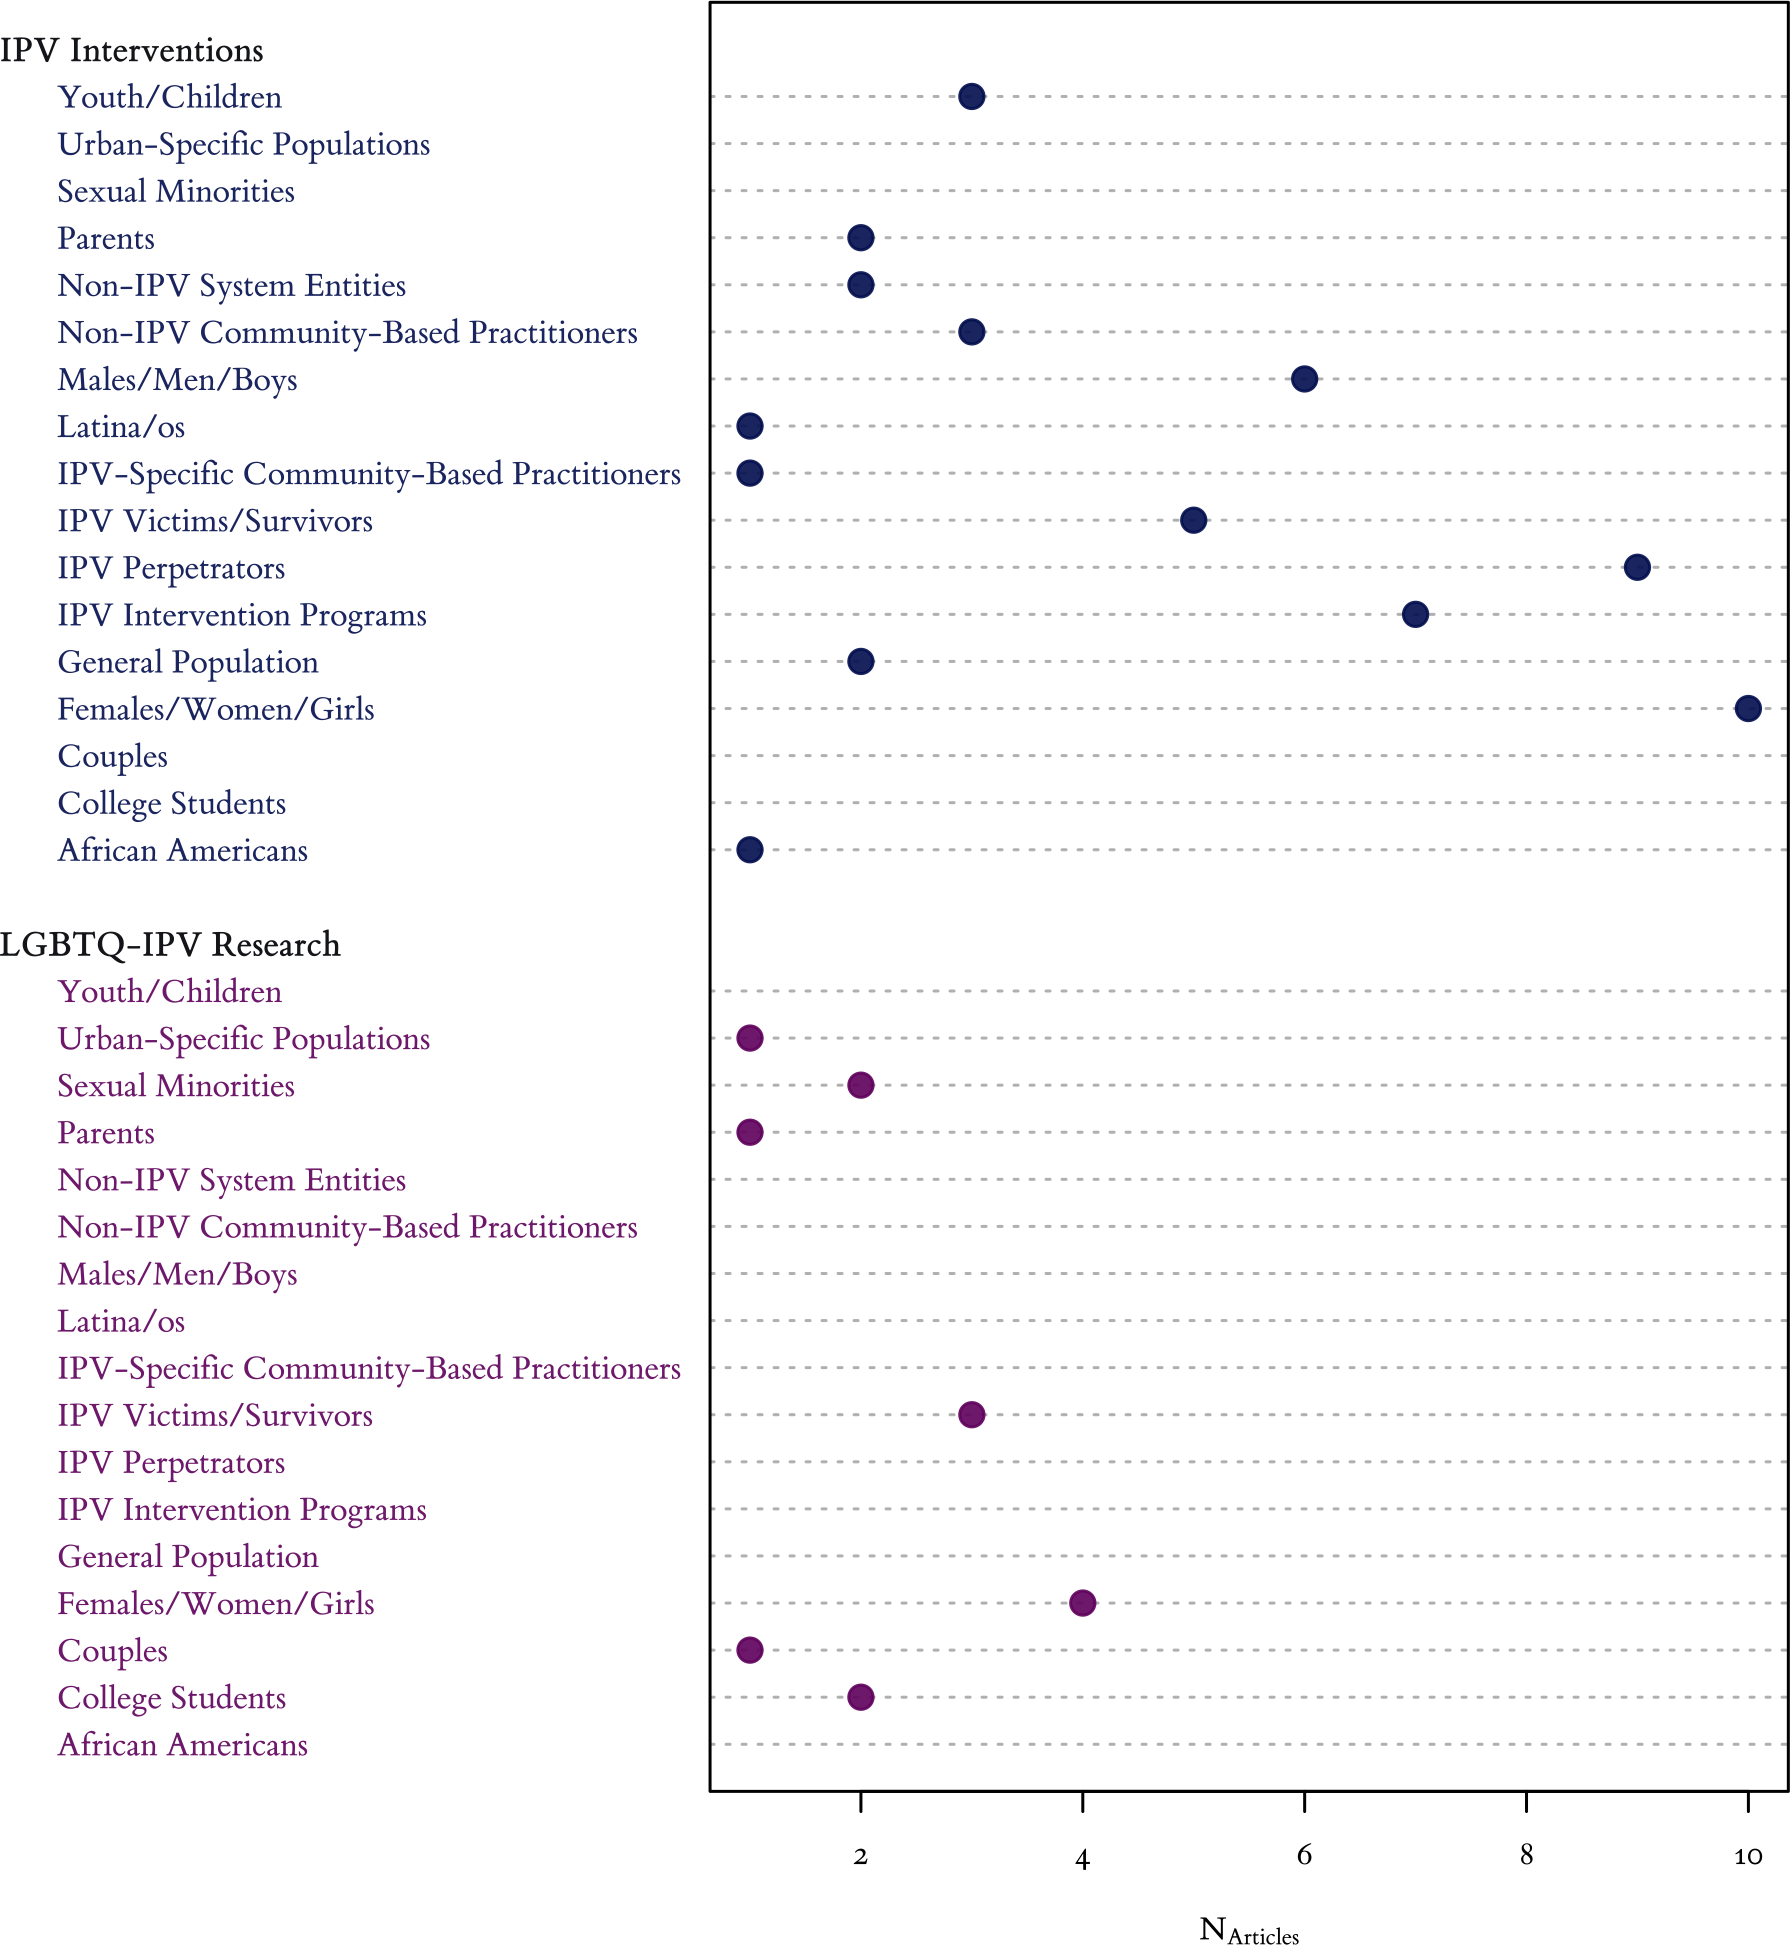
\includegraphics[width=\linewidth]{graphics/rplot-populations-1} \includegraphics[width=\linewidth]{graphics/rplot-populations-2} \includegraphics[width=\linewidth]{graphics/rplot-populations-3} \end{figure*}

\newpage

\subsection{IPV Interventions
Research}\label{ipv-interventions-research}

\begin{longtable}[]{@{}lr@{}}
\caption{Primary Topics}\tabularnewline
\toprule
& \(N_{Articles}\)\tabularnewline
\midrule
\endfirsthead
\toprule
& \(N_{Articles}\)\tabularnewline
\midrule
\endhead
Approach Evaluation & 1\tabularnewline
Coordinated Community Response & 1\tabularnewline
Int. - Description & 2\tabularnewline
Int. - Proposal & 2\tabularnewline
Measures & 1\tabularnewline
Program Evaluation Methods & 2\tabularnewline
Program/Policy Development & 3\tabularnewline
Intervention Providers' Perspectives & 1\tabularnewline
Victims'/Survivors' Perspectives & 2\tabularnewline
Program/Policy Evaluation - General & 18\tabularnewline
Public Policy & 2\tabularnewline
System Response & 2\tabularnewline
\bottomrule
\end{longtable}

\begin{longtable}[]{@{}lr@{}}
\caption{Sampling Frames}\tabularnewline
\toprule
& \(N_{Articles}\)\tabularnewline
\midrule
\endfirsthead
\toprule
& \(N_{Articles}\)\tabularnewline
\midrule
\endhead
African Americans & 1\tabularnewline
Females/Women/Girls & 9\tabularnewline
General Population & 1\tabularnewline
IPV-Perpetrators & 8\tabularnewline
IPV-Victims/Survivors & 4\tabularnewline
Latinos/Latinas or Hispanic-Americans & 1\tabularnewline
Males/Men/Boys & 6\tabularnewline
Community-Based Practitioners & 3\tabularnewline
IPV-Specific Community-Based Practitioners & 1\tabularnewline
IPV Intervention Programs & 6\tabularnewline
Parents & 2\tabularnewline
System Entities & 1\tabularnewline
Children/Youth & 4\tabularnewline
\bottomrule
\end{longtable}

\begin{longtable}[]{@{}lr@{}}
\caption{Overarching Methodology}\tabularnewline
\toprule
& \(N_{Articles}\)\tabularnewline
\midrule
\endfirsthead
\toprule
& \(N_{Articles}\)\tabularnewline
\midrule
\endhead
Mixed-Methods & 2\tabularnewline
Qualitative & 6\tabularnewline
Quantitative & 14\tabularnewline
\bottomrule
\end{longtable}

\begin{longtable}[]{@{}lr@{}}
\caption{Qualitative Methods}\tabularnewline
\toprule
& \(N_{Articles}\)\tabularnewline
\midrule
\endfirsthead
\toprule
& \(N_{Articles}\)\tabularnewline
\midrule
\endhead
Group Interviews & 4\tabularnewline
Multiple Qualitative Methods & 1\tabularnewline
Qualitative Survey & 1\tabularnewline
\bottomrule
\end{longtable}

\begin{longtable}[]{@{}lr@{}}
\caption{Quantitative Methods}\tabularnewline
\toprule
& \(N_{Articles}\)\tabularnewline
\midrule
\endfirsthead
\toprule
& \(N_{Articles}\)\tabularnewline
\midrule
\endhead
Secondary/Archival Data & 2\tabularnewline
Experimental Design & 12\tabularnewline
Longitudinal & 12\tabularnewline
Multiple Quantitative Methods & 2\tabularnewline
Intervention Providers' Perspectives & 1\tabularnewline
Client Records & 3\tabularnewline
Police Records & 2\tabularnewline
Quantitative Survey & 13\tabularnewline
Cross-Sectional & 2\tabularnewline
\bottomrule
\end{longtable}

\begin{longtable}[]{@{}lr@{}}
\caption{Mixed-Methods}\tabularnewline
\toprule
& \(N_{Articles}\)\tabularnewline
\midrule
\endfirsthead
\toprule
& \(N_{Articles}\)\tabularnewline
\midrule
\endhead
Focus Groups & 2\tabularnewline
Longitudinal & 1\tabularnewline
Quantitative Survey & 2\tabularnewline
\bottomrule
\end{longtable}

\newpage

\subsection{LGBTQ-IPV Research}\label{lgbtq-ipv-research}

\begin{longtable}[]{@{}lr@{}}
\caption{Primary Topics}\tabularnewline
\toprule
& \(N_{Articles}\)\tabularnewline
\midrule
\endfirsthead
\toprule
& \(N_{Articles}\)\tabularnewline
\midrule
\endhead
Community Capacity & 1\tabularnewline
Coordinated Community Response & 1\tabularnewline
IPV Consequences & 3\tabularnewline
IPV Dynamics & 6\tabularnewline
Help-Seeking & 2\tabularnewline
IPV Interventions (Int.) - General & 1\tabularnewline
Measures & 2\tabularnewline
Perpetrator Characteristics & 2\tabularnewline
Outsiders' Perspectives & 6\tabularnewline
Key Stakeholders' Persepctives & 1\tabularnewline
Victims'/Survivors' Perspectives & 1\tabularnewline
Protective Factors & 1\tabularnewline
IPV Prevalence & 13\tabularnewline
Risk Factors & 15\tabularnewline
System Response & 2\tabularnewline
\bottomrule
\end{longtable}

\begin{longtable}[]{@{}lr@{}}
\caption{Populations Included}\tabularnewline
\toprule
& \(N_{Articles}\)\tabularnewline
\midrule
\endfirsthead
\toprule
& \(N_{Articles}\)\tabularnewline
\midrule
\endhead
African Americans & 1\tabularnewline
`At Risk' Populations & 1\tabularnewline
Asian Americans & 2\tabularnewline
Cis-Gender & 1\tabularnewline
College Students & 5\tabularnewline
Couples & 2\tabularnewline
Non-IPV Crime Victims & 1\tabularnewline
Disabled Persons & 1\tabularnewline
Females/Women/Girls & 14\tabularnewline
General Population & 2\tabularnewline
Graduate Students & 1\tabularnewline
Heterosexuals & 4\tabularnewline
IPV-Perpetrators & 3\tabularnewline
IPV-Victims/Survivors & 7\tabularnewline
Males/Men/Boys & 5\tabularnewline
Community-Based Practitioners & 2\tabularnewline
IPV-Specific Community-Based Practitioners & 1\tabularnewline
Parents & 2\tabularnewline
Racial Minorities & 4\tabularnewline
Sexual Minorities (SM) & 7\tabularnewline
SM - Bisexuals & 4\tabularnewline
SM - Gay & 5\tabularnewline
SM - Lesbian & 13\tabularnewline
SM - Queer & 1\tabularnewline
SM - Transgender & 1\tabularnewline
System Entities & 2\tabularnewline
Urban-Specific & 1\tabularnewline
Children/Youth & 6\tabularnewline
\bottomrule
\end{longtable}

\begin{longtable}[]{@{}lr@{}}
\caption{Overarching Methodology}\tabularnewline
\toprule
& \(N_{Articles}\)\tabularnewline
\midrule
\endfirsthead
\toprule
& \(N_{Articles}\)\tabularnewline
\midrule
\endhead
Mixed-Methods & 6\tabularnewline
Qualitative & 8\tabularnewline
Quantitative & 28\tabularnewline
\bottomrule
\end{longtable}

\begin{longtable}[]{@{}lr@{}}
\caption{Qualitative Methods}\tabularnewline
\toprule
& \(N_{Articles}\)\tabularnewline
\midrule
\endfirsthead
\toprule
& \(N_{Articles}\)\tabularnewline
\midrule
\endhead
Case Study & 1\tabularnewline
Focus Groups & 2\tabularnewline
Group Interviews & 6\tabularnewline
1-on-1 Interviews & 1\tabularnewline
Multiple Qualitative Methods & 1\tabularnewline
\bottomrule
\end{longtable}

\begin{longtable}[]{@{}lr@{}}
\caption{Quantitative Methods}\tabularnewline
\toprule
& \(N_{Articles}\)\tabularnewline
\midrule
\endfirsthead
\toprule
& \(N_{Articles}\)\tabularnewline
\midrule
\endhead
Secondary/Archival Data & 8\tabularnewline
Experimental Design & 1\tabularnewline
Police Records & 3\tabularnewline
Quantitative Survey & 26\tabularnewline
Cross-Sectional & 27\tabularnewline
\bottomrule
\end{longtable}

\begin{longtable}[]{@{}lr@{}}
\caption{Mixed-Methods}\tabularnewline
\toprule
& \(N_{Articles}\)\tabularnewline
\midrule
\endfirsthead
\toprule
& \(N_{Articles}\)\tabularnewline
\midrule
\endhead
Experimental Design & 2\tabularnewline
Focus Groups & 4\tabularnewline
Group Interviews & 2\tabularnewline
Longitudinal & 2\tabularnewline
Qualitative Survey & 2\tabularnewline
Quantitative Survey & 6\tabularnewline
Cross-Sectional & 2\tabularnewline
\bottomrule
\end{longtable}



\end{document}
